%%%%%%%%%%%%%%%%%%%%%%%%%%%%%%%%%%%%%%%%%%%%%%%%%%%%%%%%%%%%%%%%%%%%%%%%%%%%%%%%
%2345678901234567890123456789012345678901234567890123456789012345678901234567890
%        1         2         3         4         5         6         7         8
\documentclass[10pt,twocolumn,letterpaper]{article}  % Comment this line out if you need a4paper

%\documentclass[a4paper, 10pt, conference]{ieeeconf}      % Use this line for a4 paper

%\IEEEoverridecommandlockouts                              % This command is only needed if 
                                                          % you want to use the \thanks command

%\overrideIEEEmargins                                      % Needed to meet printer requirements.

% See the \addtolength command later in the file to balance the column lengths
% on the last page of the document

% The following packages can be found on http:\\www.ctan.org
\usepackage{graphics} % for pdf, bitmapped graphics files
\usepackage{graphicx} 
\usepackage{epsfig} % for postscript graphics files
\usepackage{mathptmx} % assumes new font selection scheme installed
\usepackage{times} % assumes new font selection scheme installed
\usepackage{amsmath} % assumes amsmath package installed
\usepackage{amssymb}  % assumes amsmath package installed
\usepackage{array}
\usepackage{hyperref}
\usepackage{blindtext}
\usepackage{subcaption}
\newcommand{\figref}[1]{\figurename~\ref{#1}}
\newcolumntype{C}[1]{>{\centering}m{#1}}
%\usepackage[T1]{fontenc}
%\usepackage[font=small,labelfont=bf,tableposition=top]{caption}
\usepackage{floatrow}
% Table float box with bottom caption, box width adjusted to content
\newfloatcommand{capbtabbox}{table}[][\FBwidth]

\usepackage[most]{tcolorbox}
\usepackage{subcaption}
\usepackage{float}
\captionsetup[subfigure]{labelformat = parens, labelsep = space, font = small}

\usepackage{blindtext}
\DeclareCaptionLabelFormat{andtable}{#1~#2  \&  \tablename~\thetable}
%


\usepackage{multirow}
\usepackage{dsfont}

\usepackage{xcolor}
\usepackage{color}

% package for algorithm
\usepackage[linesnumbered,ruled,vlined]{algorithm2e}


%\usepackage[backend=bibtex]{biblatex}

\usepackage{graphicx} % Required for the inclusion of images
\usepackage{listings}% add c++ code

\usepackage{tabularx,ragged2e,booktabs,caption}
\usepackage{cite}

\title{\LARGE \bf
Static-map and Dynamic Object Reconstruction in Outdoor Environments using 3D Motion Segmentation }


\author{Cansen Jiang$^{1}$, Danda Pani Paudel, Yohan Fougerolle, David Fofi and C\'edric Demonceaux \\
Universit\'e de Bourgogne Franche-Comt\'e\\
12 rue de la Fonderie, 71200 Le Creusot\\} % <-this % stops a space
%%\thanks{*This work was not supported by any organization}% <-this % stops a space
%\thanks{$^{1}$ C. Jiang, D.P. Paudel, Y. Fougerolle, D. Fofi and C. Demonceaux, with the Laboratoire Electronique, Informatique et Image (Le2i) of University of Burgundy, France 
%       {\tt\small firstname.lastname@u-bourgogne.fr} }
%%\thanks{$^{2}$ Anonymous ...
%%       {\tt\small Anonymous@ieee.org}
%
%%}


%\author{Cansen Jiang, Danda Pani Paudel, Yohan Fougerolle, David Fofi and C\'edric Demonceaux % <-this % stops a space
%\thanks{*This work was not supported by any organization}% <-this % stops a space
%\thanks{ Cansen Jiang, Danda Pani Paudel, Yohan Fougerolle, David Fofi and C\'edric Demonceaux are from Le2i, Universit\'e de Bourgogne, France.
%       {\tt\small firstname.lastname@u-bourgogne.fr} }%
%\thanks{$^{2}$ Anonymous ...
%       {\tt\small Anonymous@ieee.org}}%
%}


\makeatletter
\renewcommand{\@algocf@capt@plain}{above}% formerly {bottom}
\makeatother
\def\NoNumber#1{{\def\alglinenumber##1{}\State #1}\addtocounter{ALG@line}{-1}}
\begin{document}


\maketitle
\thispagestyle{empty}
\pagestyle{empty}


%%%%%%%%%%%%%%%%%%%%%%%%%%%%%%%%%%%%%%%%%%%%%%%%%%%%%%%%%%%%%%%%%%%%%%%%%%%%%%%%
\begin{abstract}
This paper aims to build the static-map of a dynamic scene using a mobile robot equipped with 3D sensor. The sought static-map consists of only the static scene parts, which has a potential of playing a vital role in scene understanding and landmark based navigation. Building static-map requires the categorization of moving and static objects in the scene.  In this work, we propose a Sparse Subspace Clustering –based Motion Segmentation method that categories the static scene parts and the multiple moving objects using their 3D motion trajectories.  Our motion segmentation method uses the raw trajectory data, allowing the objects to move in exact 3D space, without any projection model assumption or whatsoever. We also propose a complete pipeline for static-map building which estimates the inter-frame motion parameters by exploiting the minimal 3-point Random Sample Consensus algorithm on the feature correspondences only from the static scene parts.  The proposed method has been especially designed and tested for large scene in real outdoor environments. On one hand, our 3D Motion Segmentation approach outperforms its 2D based counterparts, for extensive experiments on KITTI dataset. On the other hand, separately reconstructed static-maps and moving objects for various dynamic scenes are very satisfactory.

\end{abstract}


%%%%%%%%%%%%%%%%%%%%%%%%%%%%%%%%%%%%%%%%%%%%%%%%%%%%%%%%%%%%%%%%%%%%%%%%%%%%%%%%
\section{INTRODUCTION}
In recent years, visual Simultaneously Localization and Mapping (vSLAM) based autonomous robot navigation techniques have achieved great success in static environments. Yet, in a dynamic scene, the navigation still remains very challenging, mainly because the moving objects contribute to a poor localization accuracy and map artifacts. Under such circumstances, the localization is usually performed by estimating the camera motion based on either the features’ motion consensus \cite{c_1} or the weighted cost minimization \cite{c_2}. Dynamic scene parts in both cases are treated as alien objects or outliers, and thus discarded. However, when a significant number of features belong to the dynamic scene parts, it can not only become difficult to discard them, but also degrade the localization accuracy\cite{c0}. Therefore, robot navigation in dynamic environments requires the detection and removal of moving objects, prior to the static-map building. A static-map of the dynamic scene consists of only the static scene parts, which in itself, is a primary interest of scene modelling. Furthermore, it is also an important step towards scene understanding and landmark based navigation. Therefore, we propose a complete pipeline, see Fig.\ref{fig:pipeline}, which involves three main stages: a) 3D feature trajectories construction; b) Motion Segmentation (MS); c) 3D scene registration.

For mobile robots capturing the dynamic scene, both static and dynamic scene parts appear to be moving. Therefore, a straightforward approach to distinguish the dynamic and static parts would be to analyze their motion trajectories. In this regard, the scene parts that reciprocate the robot motion are considered to be static, whereas the remaining ones belong to the moving objects or outliers. Note that a common practice for the detection of the object motion is to segment their features' trajectories. When the robot is equipped with 3D sensors, it must be obvious to represent and segment the features' trajectories directly in 3D space. In practice, such feature trajectories can be obtained by detecting and tracking 3D feature points. If both 2D cameras and 3D sensors are available, 3D feature tracking can also be supported by their 2D feature descriptors, after projecting onto the image. In this work, a 2D optical-flow based method has been adopted to acquire the 3D feature trajectories. However, in many practical scenarios, the trajectories obtained in this manner yield numerical instability due to the non-uniform distribution on static and dynamic objects. We tackle this problem by employing a flow-likelihood based feature sampling technique so that the feature distribution on moving and static objects is balanced, making it suitable for wide range of dynamic object coverage.

\begin{figure}
  \centering
 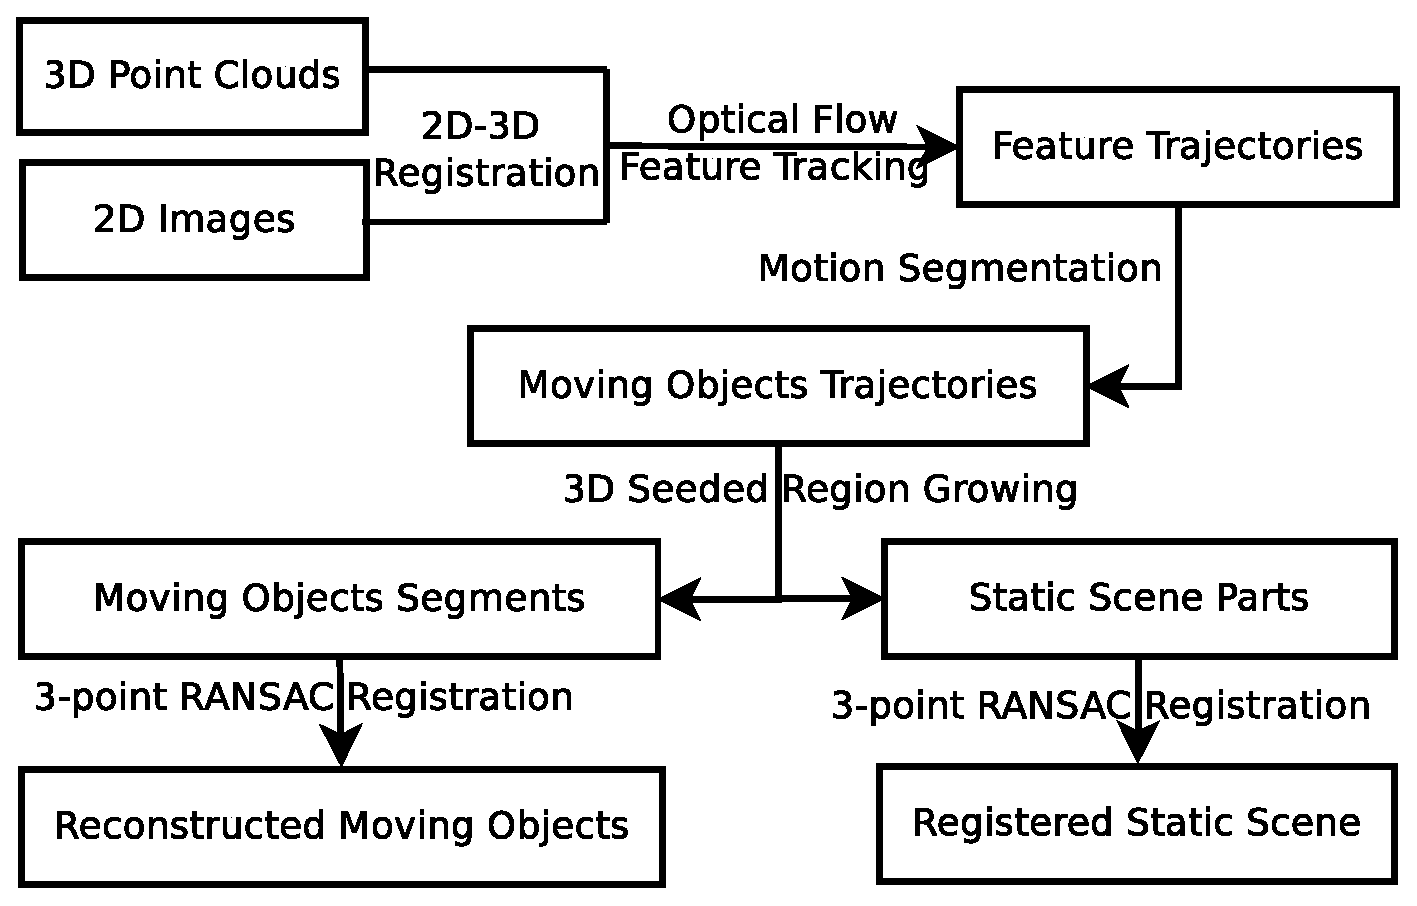
\includegraphics[width=0.8\textwidth]{image/pipeline.eps} 
		   \caption{Static-map building framework.}
  		 \label{fig:pipeline}    
\end{figure}

Starting from the 3D trajectories of sparse feature points, we propose a Sparse Subspace Clustering based 3D (3D-SSC) MS algorithm that categorizes multiple moving objects as well as the static scene parts. Although many MS methods are available in the context of video surveillance, object tracking, and action recognition \cite{c1}, they offer the solution for objects moving either in 2D space, or in 3D space under the camera projection model assumption. Our proposed method performs the motion segmentation in 3D space using raw motion trajectories, without any projection model assumption or whatsoever. The 3D-SSC algorithm intents to find the minimal linear sparse subspaces that best represent the given motion trajectories. In this work, we show with several experiments that our 3D Motion Segmentation approach outperforms its 2D based counterparts.

While building the static-map, the dynamic objects must be segmented and removed from the scene, such that only the static parts remain in the resulting map. Thanks to MS, the sparse set of feature points are divided into multiple subsets -- each subset is assigned to one object with unique motion trajectory. These feature subsets are later used to obtain dense segmentation by employing a Region Growing technique on the complete 3D scene points. Once the static parts and moving objects are detected, we have developed two applications, namely, static-map building and moving object reconstruction.  On the one side, the static-map is built by registering multi-frame point clouds. This is carried out by using minimal 3-point Random Sample Consensus (RANSAC) algorithm on the feature correspondences only from the static scene parts. The minimal 3-point RANSAC uses Cayley representation of the rotation matrix, which allows us to obtain rigid transformation between two point clouds using linear solvers, similar to \cite{c23}. The proposed static-map building algorithm performs very satisfactorily on realistic outdoor environments. On the other side, the moving objects are densely reconstructed by registering their observations from different view-ports. In addition, segmented motion trajectory facilitates us to understand the object behaviours, such as driving cars or walking pedestrians. 

The main contributions of this paper are two-folded:
\begin{itemize}
\item{A novel framework in 3D motion segmentation has been proposed. The 3D feature trajectories are grouped by applying our 3D data based Sparse Subspace Clustering algorithm which outperforms its 2D based counterparts.} 
\item{A complete pipeline in building static-map taking the advantage of motion segmentation is presented. Our system not only provides a static-map constructed from a real outdoor scene, but also better 3D reconstructions of moving objects.}
\end{itemize}


\section{Related Work}
\label{relatedWork}
%\subsection{Motion Segmentation}
For decades, numerous works have been conducted in image based motion segmentation \cite{c1}. The representative approaches, namely Generalized Principle Component Analysis (GPCA)~\cite{c9}, RANSAC-based MS~\cite{c16}, Agglomerative Subspace Clustering(ASC)~\cite{c6} and the Sparse Subspace Clustering (SSC)~\cite{c2} are intensively studied in \cite{c1}. Usually, the problem of MS is addressed by separating the motions into subspaces such that every motion trajectory belongs to its corresponding subspace. In this regard, GPCA estimates the global linear subspaces for motion clustering, while the LSA does the same locally. Although these methods provide great insight for subspace-based motions clustering, their practical usage is limited either because of their high sensitivity to noise/outliers or sharp increase in computational complexity with the increasing number of moving objects. Moreover, the RANSAC framework introduced to offer robustness in such cases is also limited, because of the rapid decrease in inliers finding  probability as the number of motions increases. ASC, a more robust method, combines the techniques of lossy compression, rank minimization, and sparse representation. Inspired by ASC, Elhamifar and Vidal~\cite{c2} proposed an SSC algorithm that relies on the idea of \textit{self-expressive} sparse representation. In fact, SSC is considered to be the leading MS method in literature~\cite{c13}.

Apart from 2D based MS, 2D-3D or 3D  based MS methods have also been developed. A recent work of Stuckler et al.~\cite{c18} performs dense 3D motion segmentation on RGB-D data using an Expectation Maximization framework. This method, however, is designed under fixed camera assumption and tested mostly in controlled environments. Another work by Perera et al.~\cite{c21} uses Truncated Signed Distance Function to segment the moving objects based on volumetric surfaces. This algorithm is supported by the RANSAC-based MS~\cite{c16} in a greedy manner, and therefore suffers form the aforementioned problems. Differently, Sofer et al.~\cite{c19} performs 3D motion segmentation using \textit{Active Machine Learning} (AML) \cite{c20} algorithm. Despite the fact that the AML algorithm provides high classification accuracy, its application specific training data requirement makes the method cumbersome. 


Static-map building is a topic of high interest in robotics and computer vision. Wang et al.~\cite{c26} proposed a method that fulfills SLAM and Moving Objects Tracking (SLAM-MOT) simultaneously. The moving objects are detected using either their map prior or the motion consistency assumption. However, both approaches fail to handle the cases of slow motions and temporal stationary objects, such as slowly walking pedestrians. To overcome the drawbacks of SLAM-MOT, Pomerleau et al.~\cite{c27} proposed to detect the moving objects using ray-tracing technique. The spatial changes are measured in the built map, obtained after using the motion from odometry sensors refined with ICP. This method also assumes that the dynamic parts have only a small scene coverage. Similarly, Ambrus et al.~\cite{c28} proposed to maintain and update a long term spatial models for Meta-room, using Normal Distribution Transform Registration. The Meta-room is a reference static structure of an office, where new scans are registered to detect and update the dynamic objects. This method maintains the static map of an office over a long term period. However, the initial requirement of clean reference model makes this method unsuitable for unknown dynamic environments. 

\section{3D Motion Segmentation}
\label{sec:3D-SSC}
Motion segmentation aims to determine different distinctive motions from the features' motion trajectories. In this context, we assume that a mobile robot captures a sequence of point clouds of a dynamic scene consisting of multiple moving objects. We also refer to the stationary objects or background as static scene parts. Similarly, the moving objects are called dynamic scene parts. Let a set of feature points are detected and tracked across the point cloud sequence to represent the features' motion trajectories. Our objective is to group these trajectories into multiple subsets such that each subset represents  a unique motion. More specifically, for $n$ objects following distinct motions, there exist $n$ subsets (or groups) of distinct trajectories, so called subspaces. All trajectories from a subspace are linearly dependent among themselves under the rigid body motion assumption. In other words, all the feature trajectories lie in union of $n$ subspaces.  


%Under the rigid motion assumption of, feature trajectories from the same subspace are linearly dependent. Accordingly, the problem of motion segmentation reduces to finding the linear subspace of the feature trajectories. To solve this problem, we propose a 3D data based Sparse Subspace Clustering (3D-SSC) approach to segment the 3D feature trajectories to their corresponding motions.

\subsection{Motion in 3-Space}
\label{ibms}
%The rigid body transformation in 3-space is defined by $3\times3$ rotation matrix $\mathsf{R}$ and $3\times1$ translation vector $\mathsf{t}$. 
Consider $\mathsf{X}$ and $\mathsf{Y}$ are the Cartesian co-ordinate vectors of corresponding feature points in two point clouds related by a rigid body motion -- rotation $\mathsf{R}$ and translation $\mathsf{t}$. The relationship between them can be established as follows:

\begin{equation}
\label{eq:rigidBodyMotion}
 \mathsf{Y}  = 
\underset{\mathsf{T} \in {\rm I\!R}^{3 \times 4}}
{\underbrace{\left[
\begin{array}{cc} \mathsf{R} &  \mathsf{t}
\end{array}  \right]}}
\left[ \begin{array}{c} \mathsf{X} \\ 1 \end{array} \right],
\end{equation}
where $\mathsf{T}$ represents the 3-space rigid transformation matrix. Let,  $\{\mathsf{X}\}_{i=1}^{P}$ represents a set of points that belong to a single rigid body in an arbitrary reference co-ordinate frame. If the moving co-ordinate frames $\{f_j\}_{j=1}^{F}$ are related to the reference by transformations $\{\mathsf{T}_j\}_{j=1}^{F}$, all  feature points $\mathsf{Y}_{ji}$ (\textit{i.e.} $j^{th}$ feature in $i^{th}$ frame) can be expressed as:
\begin{equation}
\scriptsize
\underset{Y \in {\rm I\!R}^{3F \times P} } {\underbrace{ \left[
\begin{array}{cccc} \mathsf{Y}_{11} \!&\! \mathsf{Y}_{12} \!&\! \cdots \!&\! \mathsf{Y}_{1P} \\
\mathsf{Y}_{21} \!&\! \mathsf{Y}_{22} \!&\! \cdots \!&\! \mathsf{Y}_{2P} \\
\vdots \!&\! \vdots \!&\!  \ddots \!&\! \vdots \\
\mathsf{Y}_{F1} \!&\! \mathsf{Y}_{F2} \!&\! \cdots \!&\! \mathsf{Y}_{FP}  \end{array} \right] } } \!=\! 
\underset{  T \in {\rm I\!R}^{3F \times 4}  } { \underbrace{ \left[ \begin{array}{c} \mathsf{T}_1 \\ \mathsf{T}_2 \\ \vdots \\ \mathsf{T}_F \end{array} \right] }}
\underset{X \in {\rm I\!R}^{4 \times P}} { \underbrace{ \left[ \begin{array}{cccc} \mathsf{X}_1 \!&\! \mathsf{X}_2 \!&\! \cdots \!&\! \mathsf{X}_P \\ 1 \!&\! 1 \!&\! \cdots \!&\! 1 \end{array} \right] }} ,
\label{eq: rigidMot}
\end{equation}
where $T$  and $X$ represent the motion and structure of a dynamic object, respectively. The columns of matrix $Y$ contain the motion trajectory of feature points. Note that the rank of $Y$ can be at most of 4. Since all the entries of $X$'s last row are one, the trajectory of feature points (\textit{i.e.} the columns of $Y$) lie in a subspace of ${\rm I\!R}^{3F}$ of dimension at most three. In case of multiple motions, say $n$, every motion must lie in the union of $n$ such subspaces. If $\{Y_k\}_{k=1}^{n}$ correspond to $n$ different unknown motions, the measurement matrix, say $Z$, containing all measured trajectories can be denoted as:
\begin{equation}
\label{eq:subSpaceToMeasurement}
Z = \left[ \begin{array}{cccc} \mathbf{z}_1 \!&\! \mathbf{z}_2 \!&\! \cdots \!&\! \mathbf{z}_m \end{array} \right] = 
\left[ \begin{array}{cccc} Y_1 \!&\! Y_2 \!&\! \cdots \!&\! Y_n \end{array} \right]\mathsf{C},
\end{equation}
where  $\mathsf{C} \in {\rm I\!R}^{m \times m} $ is an unknown permutation matrix. Equation~\eqref{eq:subSpaceToMeasurement} shows that the measured trajectories $\{\mathbf{z}_l\}_{l=1}^{m}$ lie in the union of $n$ subspaces. 

\subsection{Sparse Subspace Representation and Recovery}
Referring to the Equation~\eqref{eq:subSpaceToMeasurement}, one can observe that the problem of 3D motion segmentation reduces to that of decomposing $Z$ into $\{Y_k\}_{k=1}^{n}$ and $\mathsf{C}$. This problem is addressed in \cite{c2} by solving a relaxed optimization problem, using the self-expressiveness property of the data. The solution is obtained under the assumption that every $\mathbf{z}_i$ can be represented as a combination of the columns of $Z$ with $\mathbf{z}_i$ removed. To make the representation least ambiguous, the combination coefficients are made as sparse as possible. Such solution is refereed as subspace-sparse representation (SSR). Therefore, a relaxed optimization problem for SSR can be written as:


\begin{equation}
\label{eq: SSR_1}
 \text{min}\, {\parallel \mathsf{C} \parallel}_1,\,\, \text{s.t.}\, \ Z=Z\mathsf{C},\,\, \text{diag}(\mathsf{C})=0.
\end{equation}

Although this optimization problem is solved as in \cite{c2}, our formulation includes a noteworthy modification that is critical to the problem at hand: the entries of $\mathsf{C}$ are forced to be non-negative so that similar motions in opposite directions are not considered to be the same. This happens especially (but not limited to) when the observed objects are moving along the robot's direction with twist speed. Such objects get categorized as background (because of the opposite relative motions), if the non-negativity constraint is not considered. 
Furthermore, among many approaches for handling noisy data, we have adopted the most suitable technique based on our empirical evaluation. Consequently, for a $3F\times 3F$ identity matrix $\mathsf{I}_d$ and $c_{ij}$ the entries of $\mathsf{C}$, the final optimization problem is stated below:
\begin{equation}
\label{eq:SR_4}
\text{min} {\parallel \mathsf{C} \parallel}_1, \ \text{s.t.} \ Z \!=\!
\left[\!
\begin{array}{cc} Z \! & \! \mathsf{I}_d
\end{array}  \!\right]\! \mathsf{C}, \text{diag} ( \mathsf{C} )=0 , c_{ij}\geq 0.
\end{equation}
Once the sparse representation matrix $\mathsf{C}$ is computed, a weighted graph $\mathcal{G}$ with weights $\mathcal{W} =  |\mathsf{C}| + {|\mathsf{C}|}^\text{T}$ is built. The segmentation of trajectories into different subspaces is obtained by applying  spectral clustering \cite{c14} method on the Laplacian of graph $\mathcal{G}$. Alternatively, any other clustering method can be applied on graph $\mathcal{G}$ for the same task.

%Then a K-mean clustering \cite{c15} approach is applied on the symmetric similarity matrix $\mathcal{W}$ to get a block-diagonal matrix. Note that the number of subspaces can be determined by taking the number of most significant eigenvalues.

%\subsection{Sparse Subspace Recovery}

\subsection{The Algorithm}
\label{ssc}

The proposed 3D motion segmentation algorithm (3D-SSC) is an extension of the existing image based SSC (2D-SSC), readers are strongly recommended to refer \cite{c2} for its theoretical derivations. For implementation aspects, our system is designed based on the 2D-SSC toolbox \cite{c2}, with the following critical modifications: a)~A modified system with 3D data based-SSC; b)~Non-negative constrain in sparse representation to distinguish similar motions in opposite directions; c)~Diagonal identity constrain (see Equation~\eqref{eq:SR_4}) adoption for corrupted data recovery. The structured work-flow for 3D-SSC implementation is illustrated in Algorithm~\ref{alg:algo1}. Such system offers the following advantages: 
\begin{list}{\labelitemi}{\leftmargin=1em}
\item Exact 3D space motion analysis: perspective effects, produced by the affine projection assumption, can be avoided.
\item More precise motion behaviour analysis: object motion estimation, namely the rotation and translation, can be precisely recovered from the segmented 3D motion trajectories for each moving object.
\item Better perception of scene structure: the 3D data provide more meaningful information, e.g. geometric structures, continuity or discontinuity, for better scene understanding.
\end{list}
\begin{algorithm}
 \caption{3D-SSC Motion Segmentation.}
 \label{alg:algo1}
 \KwData{ 3D feature trajectories $Z \in R^{3F \times m}$.}
 \KwResult{ $\textit{n}$ clustered subspaces.}
 Sparse Subspace Recovery using Equation~\eqref{eq:SR_4}.
 
 Similarity Graph: $\mathcal{G}$ with $\mathcal{W} =  |C| + {|C|}^\text{T}$.
 
 Spectral Clustering on $\mathcal{W}$.

\end{algorithm}




\section{Static-map Building}
%\subsection{System setup}
For controlled environments, one can safely assume that the static-map can always be built after physically removing the dynamic object from the scene, or by restricting them to move while building the map. However in the real-world outdoor scenes, it is very often impractical to restrict the objects to move, such as driving cars and walking pedestrians, for the sake of map building. A common practice  involves the selection of right time frame so that the number of moving objects are minimized. Any act of leveraging form this restriction makes the presence of dynamic objects unavoidable. In such scenarios, the process of static-map reconstruction demands the detection and the removal of dynamic objects while building the map, or preferably before.

To reconstruct a static-map in an outdoor environment, we suggest to use a mobile robot equipped with both 2D camera and 3D sensor. Ideally, a 3D sensor alone is sufficient for the proposed static-map building framework. However in practice, construction of meaningful trajectories using only 3D data is undermined by the lack of robust 3D feature descriptors. Therefore, we also make use of the 2D camera -- calibrated and synchronized with 3D sensor, sharing the same field of view. Although the RGB-D camera is a good example of this kind, any combination of 2D camera and 3D sensor would suffice as long as the aforementioned criteria are satisfied. Doing so, allows us to associate 3D points to their 2D descriptors, by projecting them  onto the image plane. The process of feature trajectory construction is followed by our 3D MS method as proposed in Section~\ref{sec:3D-SSC}. The point clouds of the static scene parts are later obtained after performing region growing on the segmented motion trajectories. Finally, the static-map is built by registering these point clouds with the help of RANSAC. The complete pipeline of the proposed static-map building method is depicted in Fig.~\ref{fig:pipeline}.   
   
 
 % Ideally, the 3D point cloud acquired from 3D sensor should contains no moving object, such that the registered 3D point cloud produces a static-map. However, in a real-world, moving objects such as driving cars or walking pedestrians, are unavoidable. Therefore, moving objects should be detected and removed from the 3D point cloud before conducting the registration. For this purpose, we present a complete pipeline with a as depicted in Fig.\ref{fig:pipeline}, to tackle this challenge. 
  
  %Note that our system requires both 2D and 3D sensors to be calibrated and synchronized, so that the image and the 3D point cloud can be registered by directly projecting the 3D point cloud onto the 2D image plane.
%\begin{figure}[!h]
%  \centering
%   \parbox{3in}{
%		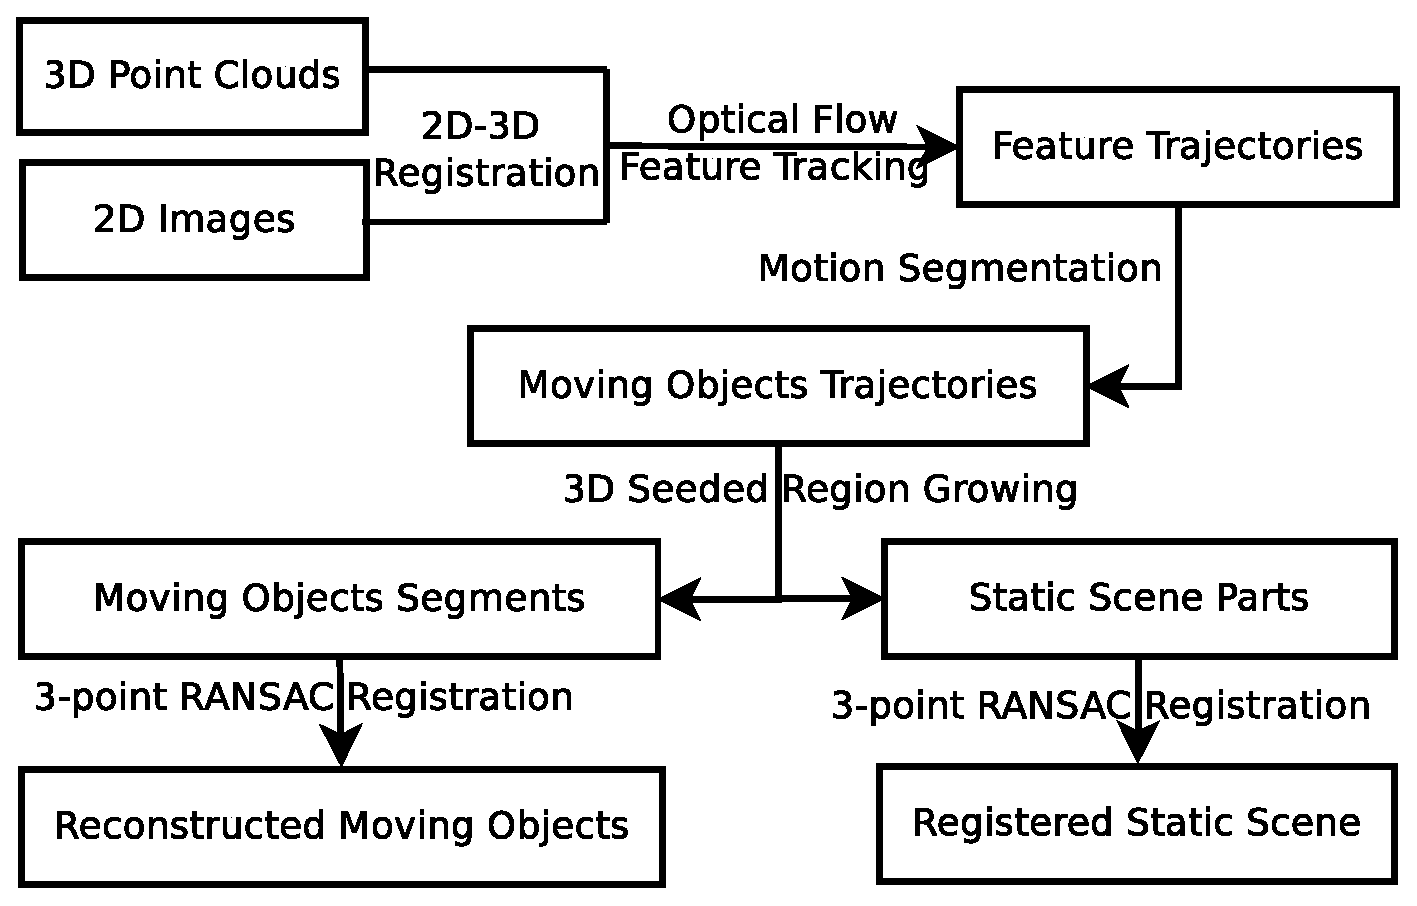
\includegraphics[width=1\textwidth]{image/pipeline.eps}      
%      }
%   \caption{Static-map building framework.}
%   \label{fig:pipeline}
%\end{figure}

\subsection{Feature trajectory Construction and Segmentation}
The feature trajectories are constructed using both 2D and 3D measurements. First, we project  all 3D scene points of the reference frame onto its image.  These projections are considered as 2D feature points and tracked across the image sequence using  a dense optical flow method.  To cover a wide speed range, coarse-to-fine dense Optical Flow \cite{c24} tracking algorithm has been adopted. The 3D feature trajectories are then retrieved from 2D feature trajectories, after establishing 2D-to-3D correspondences similar to \cite{c31}. We refer dynamic coverage to the area that the dynamic objects cover in an image. Our primary interest is to perform robust MS, while addressing a wide range of dynamic coverage as well as the speed. For example, if the dynamic object covers a small part of the image or quickly changes its apprentice because of the high speed, only a small fraction of tracked features belong to this object. This makes the data highly imbalanced, causing the numerical instability during subspace-sparse representation. To addressed this problem, we introduce a flow likelihood-based sampling of the trajectories. Let $\{\mathbf{v}_l\}_{l=1}^m$ are the measured speeds corresponding to the  trajectories $\{\mathbf{z}_l\}_{l=1}^m$ (refer Equation~\eqref{eq:subSpaceToMeasurement}). If $\{c_l\}_{l=1}^m$ are the binary classes (dynamic=1, and static = 0) assigned to each trajectory, the likelihood function is defined as
\begin{equation}
\label{eq: likelihood}
\mathcal{L}(c_l=1|Z) = e^{{\parallel \mathbf{v}_l - \mathbf{ \bar{v}} \parallel}^2/ {\sigma^2} },
\end{equation}   
where $\mathbf{ \bar{v}}$ and $\sigma$ are the median speed and standard deviation respectively. A subset of feature trajectories for MS are selected based on the likelihood measure of Equation~\eqref{eq: likelihood}. This sampling method avoids the problem of having too many samples from the background, hence balancing the data for the optimization problem of Equation~\eqref{eq:SR_4}. 

Once the segmented feature trajectories are obtained, a multi-seeded Region Growing \cite{c25} technique is applied on the point clouds to densely segment the moving objects in the scene. After segmenting all the dynamic objects,  remaining point clouds represent the static scene parts.


\subsection{3-point RANSAC Registration}
Given the segmented point clouds, the static-map is built by registering multiple point clouds of the static parts. The registration is performed using 3-point RANSAC on rigid transformation parameters. In fact, the segmented  motion trajectories also allow us to obtain the dense reconstruction of dynamic objects in a very similar manner. Recall the rigid transformation of Equation~\eqref{eq:rigidBodyMotion}. Let $\mathsf{g}$ be Gibbs representation of a rotation matrix $\mathsf{R}$. Also, $\mathsf{G}=[\mathsf{g}]_\times$ and $\mathsf{I}_3$ are $3\times 3$ skew-symmetric and identity matrices, respectively. Using Cayley Transform~\cite{c30}, $\mathsf{R}$ can be expressed as:

\begin{equation}
\label{eq:CayleRotation}
\mathsf{R} =(\mathsf{I}_3 + \mathsf{G})^{-1} (\mathsf{I}_3 - \mathsf{G}).    
\end{equation}

Using Equation~\eqref{eq:CayleRotation}, Equation~\eqref{eq:rigidBodyMotion} can be rewritten as:
\begin{equation}
\label{eq:CayleRigidBody}
(\mathsf{I}_3 + \mathsf{G})\mathsf{Y} = (\mathsf{I}_3 - \mathsf{G})\mathsf{X}+ (\mathsf{I}_3 + \mathsf{G})\mathsf{t}.    
\end{equation}

If the second term on right hand side of Equation~\eqref{eq:CayleRigidBody} is replaced by a new vector $\tilde{\mathsf{t}}$, it can be written as
  \begin{equation}
\label{eq:CayleRigidBodyLinear}
(\mathsf{Y}-\mathsf{X}) = -(\mathsf{Y}+\mathsf{X})\mathsf{G}+ \tilde{\mathsf{t}}.    
\end{equation}
Note that the Equation~\eqref{eq:CayleRigidBodyLinear} is linear in the entries of $\mathsf{g}$ and $\tilde{\mathsf{t}}$. Each pair of corresponding points provides 2 independent equations, for a system of 6 unknowns. Therefore, only 3 correspondences are required to solve this system linearly. It is straightforward to recover $\mathsf{R}$ and $\mathsf{t}$ from its solution. 

Cayley Transform based rotation matrix representation is well known in geometry, however, its usage in robotics is shadowed due to its inability to represent the rotation of $180^{\circ}$. In fact, the Gibbs vector for rotation angle $\theta$ and axis $\hat{\mathsf{g}}$ is expressed as: $\mathsf{g}=tan(\theta/2)\hat{\mathsf{g}}$. The entries of  $\mathsf{g}$ start behaving badly from $\theta>90^{\circ}$, due to the tangent nature. For $\theta<90^{\circ}$, it can be safely used to estimate the rigid motion. On the positive side, this representation offer a linear solution using minimal 3-point correspondences. More importantly, the over-determined system constructed from all inliers, at the refinement stage of RANSAC, can be solved using linear least-square method on exact 6 rigid motion parameters. 


\section{Experiments}
\label{experiment}
To validate the proposed algorithm, both synthetic data and real data acquired using Microsoft Kinect RGB-D camera, and KITTI dataset \cite{c32} are experimented. The results show the feasibility of the proposed 3D-SSC in segmenting the 3D trajectories. Furthermore, both quantitative and qualitative results of reconstructed static-maps using the proposed method are discussed in details. All the experiments are conducted in a computer with Intel Quad Core i7-2.7GHz, 32GB Memory.

\subsection{3D-SSC MS Simulation}
We build a system that contains multiple moving objects under different noise conditions to verify the robustness of the algorithm. More specifically, a set of synthetic data are generated with $\textit{n}$ moving cubes. The $\textit{n}$ moving cubes have different sizes, positions, orientations and motions. The motion feature trajectories are randomly selected to generalize the algorithm evaluation. Note that the trajectories might be inter-crossing with each other and some feature points might be occluded during their motions. To quantify the robustness of the algorithm under different noise levels, the miss-classification rate is defined as
$\eta = \frac{\# \ \text{miss-classified features} }{ \# \ \text{total features} }$. Fig.~\ref{fig:MotSegSim} illustrates the simulation, from which a set of features trajectories are selected lying on the surface of 5 moving cubes. Initially, the feature trajectories are uncategorised, see Fig.~\ref{fig:multiMotGen}. After applying the 3D-SSC MS, the feature trajectories are clustered correctly, see Fig.~\ref{fig:multiMotGenSeg}. To test the performance of the algorithm under different noise levels and multiple motions, various levels of white noise (from ${0\%, \ 2\%, \ \cdots, \ 12\%}$) are introduced to feature locations. Fig.\ref{fig:nObjs_noise} shows that the 3D-SSC behaves very robustly under $10\%$ of noise for at least 10 moving objects.

\begin{figure}[hb]
\centering
	\begin{subfigure}{0.5\textwidth}
  	\centering
 	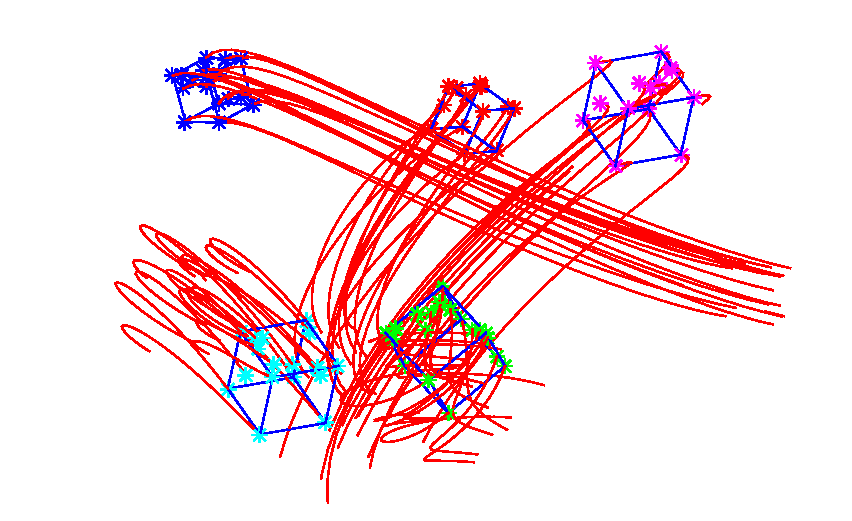
\includegraphics[height=0.1\textheight, width=0.95\textwidth]{image/multiMotGenSingle.eps}
  	\caption{Init. uncategorised motions.}
  	\label{fig:multiMotGen}
	\end{subfigure}%
	\begin{subfigure}{0.5\textwidth}
 	\centering
  	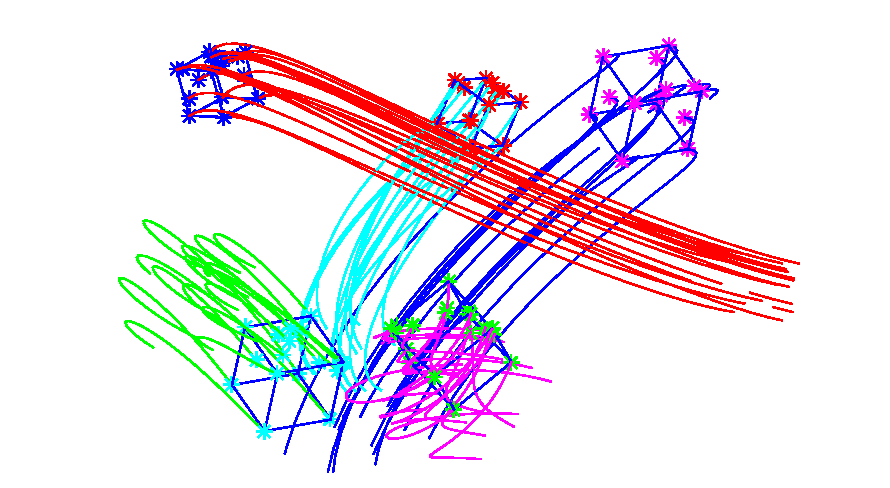
\includegraphics[height=0.1\textheight, width=0.95\textwidth]{image/multiMotGenSeg.eps}
  	\caption{3D-SSC MS result.}
  	\label{fig:multiMotGenSeg} 
  	\end{subfigure}%
  	\caption{3D-SSC MS on synthetic 3D data: (a) shows the randomly generated 5 rigid motions with uncategorised trajectories. (b) shows the 3D-SSC MS results that motions are labelled with particular colors. Must view in color.}
  	   \vspace*{-0.3cm}
   \label{fig:MotSegSim}
\end{figure}
   \vspace*{-0.3cm}

\begin{flushleft}
\begin{figure}[thpb]
		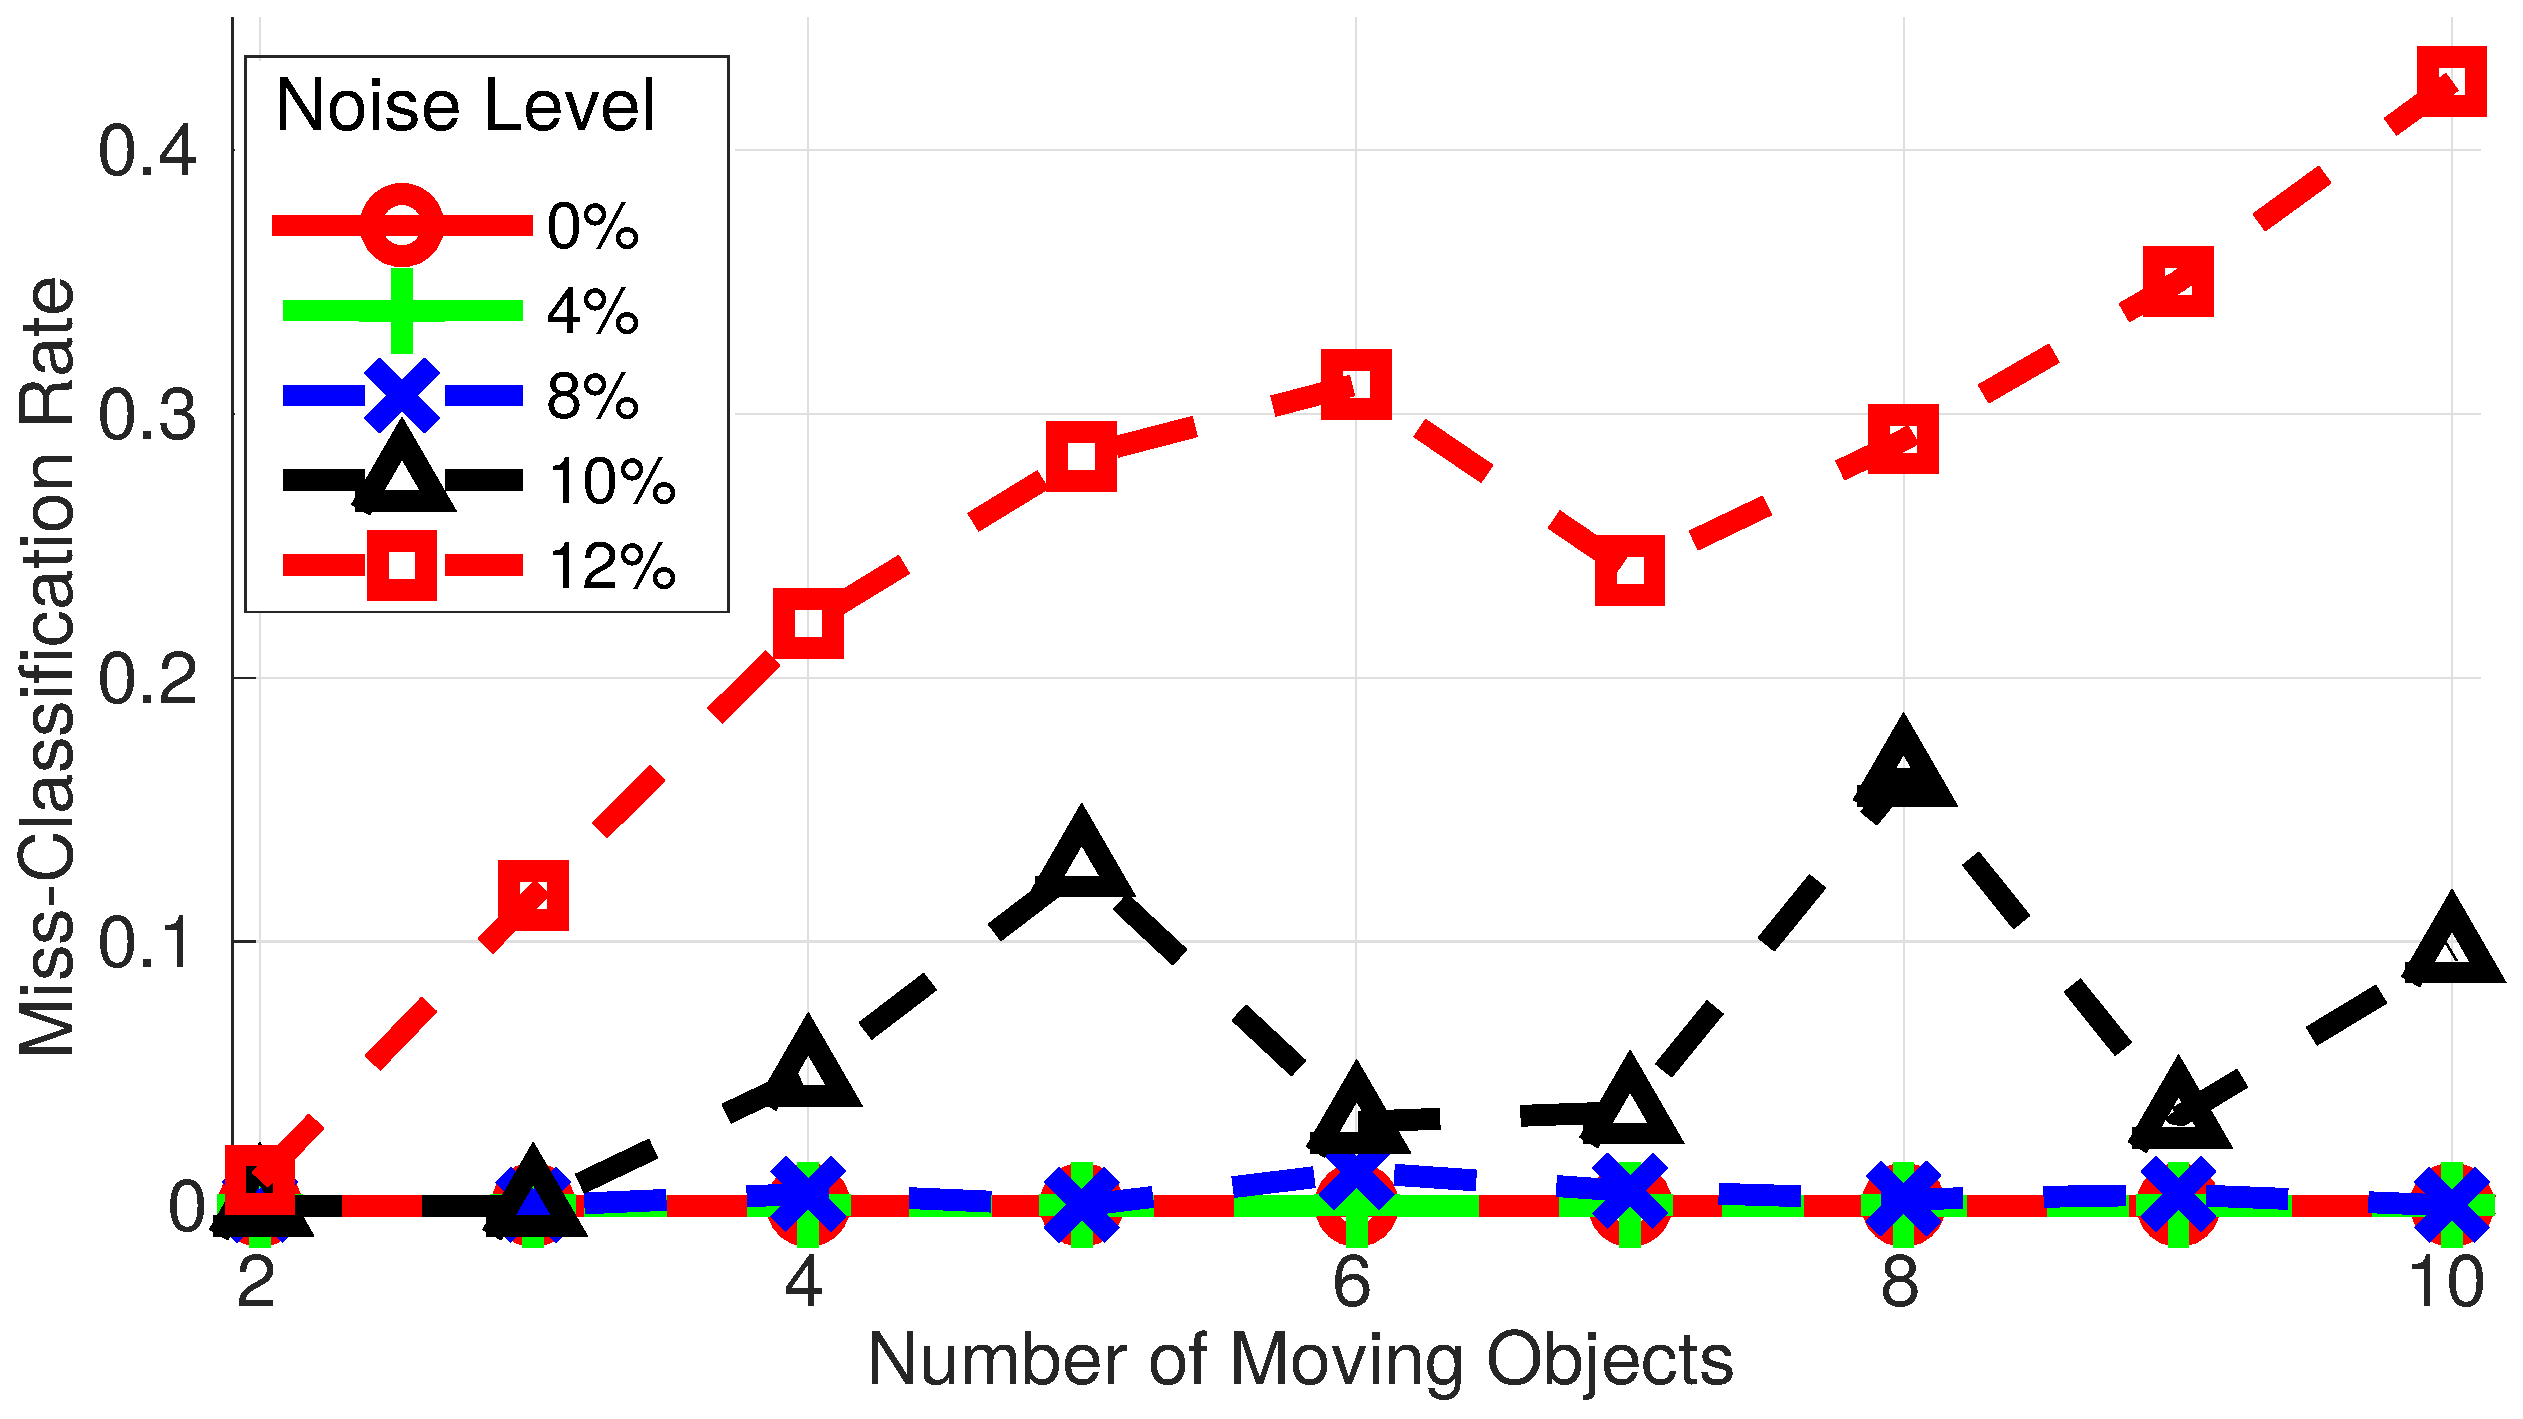
\includegraphics[width=0.85\textwidth]{image/MissClassification_nObjs_modified2.eps}      
   \caption{3D-SSC MS evaluation on $\textit{n}$ moving objects.}
   \label{fig:nObjs_noise}
   \vspace*{-0.3cm}
\end{figure}
\end{flushleft}
   \vspace*{-0.3cm}

\subsection{Evaluation using Kinect Data}
To evaluate the performance of the algorithm on real 3D data, a set of RGB-D sequence using Microsoft Kinect are recorded, see Fig.~4. In the experiment, 5 moving objects with different shapes are involved, namely the book, bottle, mug, lamp, and box. All the moving objects are attached with a chessboard pattern for the ease of feature selection and annotation. The details of the experiments are summarized in Table~I, where the columns represent the trajectory length, the number of features, and the segmentation accuracy ($1-\eta$), respectively. As can be seen from Table~I, the trajectories' length for different objects are different, thus representing the incomplete trajectory cases. These results show that the 3D-SSC algorithm is able to correctly and precisely segment the 3D feature trajectories in a controlled indoor environment.

% update Yohan: eps file for image
\begin{figure}[!h]
\begin{floatrow}
\ffigbox{%
  \label{fig:kinect_data}
  \includegraphics[height=.223\textwidth, width=0.4\textwidth]{image/KinectFeats.eps} %{image/KinectFeats.png} 
}{%
  \caption{Kinect data. }%
}
\hspace{-.8cm}
\capbtabbox{%
  \scriptsize
  \label{tab:kinect_ssc}
		\begin{tabular}{|C{0.58cm}|C{0.47cm}|C{0.47cm}|C{0.75cm}|}
		\hline 
		Objects &Len. & Feat. & Acc.(\%)\tabularnewline
		\hline 
		\hline 
		Mug & 15 & 18 & 100\tabularnewline
		\hline 
		Bottle & 32 & 12 & 100\tabularnewline
		\hline 
		Lamp & 24 & 18 & 100\tabularnewline
		\hline 
		Box & 22 & 18 & 100\tabularnewline
		\hline 
		Book & 20 & 16 & 93.75\tabularnewline
		\hline 
		\end{tabular}
		
}{%
  \caption{Kinect MS results.}%
}
\end{floatrow}
\vspace{-3mm}
\end{figure}


\subsection{Evaluation on KITTI Dataset}
To evaluate our system with realistic outdoor scenes, we conduct extensive experiments on the KITTI dataset \cite{c32}. The experiments are conducted with four different datasets, namely Highway, Junction, Station, and Market. These datasets have been selected with different frame lengths, number of moving objects, and number of feature trajectories. The details of all four datasets are provided in Table~\ref{tab:2d3dMScomparision}. In this table, the speed indicates the relative speed of the moving objects with respect to the camera. Note that the dynamic objects cover a wide range of speeds, representing both fast and slow motions.

\subsubsection{MS Evaluation}
The feature trajectories are constructed using the dense optical flow tracking approach and sub-sampled based on the flow-likelihood sampling technique. As can be observed in Fig.~\ref{fig:2dtraj}, a significant number of features belong to the dynamic parts, although they cover relatively small region. Such feature distribution helps to balance the data for the sparse representation, thanks to the likelihood sampling. Fig.~\ref{fig:3dtraj} shows the 3D feature trajectories. Fig.~\ref{fig:2dRG} and Fig.~\ref{fig:3dRG} show segmentation results obtained by 2D-SSC~\cite{c2} and 3D-SSC, respectively. Note that the 2D-SSC MS fails to categorize the road sign as a static scene part.

The results obtained using 2D-SSC MS as well as 3D-SSC MS for all four datasets are summarized in Table~\ref{tab:2d3dMScomparision}. The segmentation performances are assessed by the popular \textit{Sensitivity} and \textit{Specificity} metrics \cite{c33}. We also report another measurement, reported as Seg. $\geq 50\% $, counting the number objects with more than half of the feature points correctly classified. Finally, the eigenvalue ratios are computed by $\rho= \frac{\sum_{i=1}^{n}\lambda _i}{\sum_{j=1}^{m}\lambda _j}$, where $n$ and $m$ are the number of motions and the total number of trajectories, respectively. The higher value of $\rho$ denotes a better representation of the motion subspaces. The Table~\ref{tab:2d3dMScomparision} also reports the computation time for both of the methods (software developed with MATLAB).

Three main observations should be noted: a) 2D-SSC has very high sensitivity with less motions, while its performance decreases significantly as motion number increases. In contrast, the proposed 3D-SSC algorithm remains robust against abundant motions. b) The 3D-SSC results are more meaningful in the sense that even when it cannot perfectly classify all the trajectories, the motions can still be correctly categorized based on the trajectories' voting. c) The 3D-SSC performs superior to 2D-SSC due to the fact that the subspace representation based on exact 3D space is more compact than that of 2D-SSC. This can be observed from the Eigen Ratio column of Table~\ref{tab:2d3dMScomparision}.
\\

\begin{table*}
\scriptsize
\begin{tabular}{|C{0.85cm}|C{0.8cm}|C{0.7cm}|C{0.7cm}|C{0.6cm}|C{0.6cm}|C{0.65cm}|C{0.65cm}|C{0.65cm}|C{0.6cm}|C{0.6cm}|C{0.6cm}|C{0.6cm}|C{0.65cm}|C{0.65cm}|C{0.65cm}|C{0.65cm}|}
%\begin{tabular}{|c|c|c|c|c|c|c|c|c|c|c|c|c|c|c|c|}
\hline 
\multirow{2}{*}{Seq.} & \multirow{2}{*}{\# Frames} & \multirow{2}{*}{\# Objs.} & \multirow{2}{*}{\# Feat.} & \multicolumn{2}{c|}{Speed (m/s)} & \multicolumn{2}{c|}{Sensitivity} & \multicolumn{2}{c|}{Specificity} & \multicolumn{2}{c|}{ Seg. $\geq 50\% $} & \multicolumn{2}{c|}{Eigen. Ratio}& \multicolumn{2}{c|}{Time(min.)} \tabularnewline
\cline{5-16} 
 &  &  &  & Min. & Max. & 2D & 3D & 2D & 3D & 2D & 3D & 2D & 3D & 2D & 3D \tabularnewline
\hline 
\hline 
Highway & 45 & 2 & 122 & 4.87 & 7.22 & \textbf{1.0} & 0.95 & \textbf{1.0} & \textbf{1.0} & 2 & 2 & 0.0250 &0.0264 & 3.54 & 4.83\tabularnewline
\hline 
Junction & 70 & 3 & 83 & 0.50 & 5.15 & \textbf{1.0} & 0.98 & 0.77 & \textbf{0.99} & 3 & 3 & 0.0398 &0.0399 & 9.61 & 12.85 \tabularnewline
\hline 
Station & 9 & 6 & 77 & 0.35 & 7.12 & 0.62 & { \textbf{0.95}} & 0.31 & { \textbf{0.66}} & 3 & { \textbf{6}} & 0.0789& 0.0979 & 1.39 & 1.68 \tabularnewline
\hline 
Market &13& 9 & 50 & 0.39 & 1.34 & 0.88 & \textbf{1.0} & 0.68 & \textbf{0.98} & 6 & \textbf{9} &0.0666 &0.1907 & 1.61 & 2.09 \tabularnewline

\hline 
\end{tabular}
\caption{2D-SSC vs. 3D-SSC in MS on KITTI dataset.}
  \label{tab:2d3dMScomparision}
  \vspace{-3mm}
\end{table*}


\subsubsection{Static-map Evaluation}
Thanks to the effectiveness of MS, the static-maps of three dynamic scenes are reconstructed, namely the Junction, Highway, and Train station, see Fig.\ref{fig:car_static_map_Reconst}, \ref{fig:truck_static_map_Reconst}, \ref{fig:train_static_map_Reconst}. To illustrate the quality of the reconstructed static-maps, the full scene reconstructions using state-of-the-art method \cite{c31} are also shown sidewise. Few 2D frames from the sequence are also displayed for the motion visualization. In details, the Fig.\ref{fig:car_static_map_Reconst} (Junction) shows the reconstructed static-scene in a long sequence, the moving car and the cyclist are detected and segmented correctly. Though there are few frames rejected due to the loss of tracked features, the proposed system is robust enough to reconstruct a long sequence with significantly changing lightening conditions. 
 
In the Highway sequence, the qualitative analysis between Fig.~\ref{fig:truck_full_tree} and Fig.~\ref{fig:truck_static_tree} show that the static scene part of our map is significantly better than that of \cite{c31}. For instance, the red rectangle region in Fig.-left highlights the tree shadow which is barely recognized. on the contrary, the same shadow in Fig.~\ref{fig:truck_static_tree} has been recovered more realistically. In the close-up view of all the built maps, similar differences are abundant. A more challenging dataset shown in Fig.~\ref{fig:train_static_map_Reconst} (Train Station) contains fast moving car and slowly moving pedestrians, with intermittently occluded train by moving objects. Interestingly, all moving objects: pedestrians, fast driving car, and occluded train are detected and removed correctly in the reconstructed static-map (see Fig.~\ref{fig:train_static_view2}). Recall that the objects moving in the same direction with similar speed share the same motion subspace. Therefore, the car and the train are grouped together (blue objects in Fig.\ref{fig:train_MS3D_marked}), so as the two pedestrians (yellow objects in Fig.\ref{fig:train_MS3D_marked}). In fact, such motion grouping simplifies the complexity of scene understanding based on the motion behaviour. 
 
 Table~\ref{tab:static_map_quantification} summarizes the  quantification results of static-map reconstruction. Starting from the second column, they represent the amount of moving objects, the number of correctly and incorrectly removed objects, and accuracies in removing the dynamic objects and maintaining the static scene parts. A higher dynamic accuracy (Dyn. Acc.) means  a better removal of dynamic objects. Similarly, the higher static accuracy (Stc. Acc.) stands for a better maintenance of the static scene parts. Results show that the dynamic objects are removed correctly with very high accuracy, meanwhile, the static scene parts are maintained very well. The computation time is reported, including the MS time and static-map reconstruction time. 
 
\begin{table}
\scriptsize
%\begin{tabular}{|c|c|c|c|c|c|c|}
\begin{tabular}{|C{0.75cm}|C{0.9cm}|C{0.6cm}|C{0.6cm}|C{0.8cm}|C{0.8cm}|C{0.8cm}|}
\hline 
Seq. & \# Objs. & Corr. & Incorr. & Dyn. Acc.($\%$) & Stc. Acc.($\%$) & Time (min.) \tabularnewline
\hline 
\hline 
Highway & 1 & 1 & 0 & 97.55 &100 & 6.00\tabularnewline
\hline 
Junction & 2 & 2 & 0 & 91.02 &100 & 13.40\tabularnewline
\hline
Station & 5 & 5 & 1 & 91.60 &92.47 & 3.16 \tabularnewline
\hline 
\end{tabular}
\caption{Static-map quantification.}
\label{tab:static_map_quantification}
\vspace{-3mm}
\end{table}
%\vspace*{-0.5cm}
As offered by our static-map building framework, dense reconstructions of the dynamic objects are recovered using multiple frame measurements, as shown in Fig.\ref{fig:movReconst}. Firstly, Fig.~\ref{fig:leftSparse_car}-\ref{fig:rightDense_car} show two views of the denser reconstruction of a car along with their single frame representations. Secondly, Fig.\ref{fig:truck_traj} shows the multi-frame grouping of the truck's point clouds in a common co-ordinate frame, obtained using [34]. It goes without saying that this representation can hardly be identified as a truck. On the contrary, the reconstructed truck using our method has very high quality, see Fig.~\ref{fig:truck_side_bright}-\ref{fig:truck_top_bright}. Thirdly, the full reconstruction of the moving train is shown in Fig.\ref{fig:train_top} obtained from its partial measurement due to dynamic occlusions at all time. 

%update Yohan : files in eps format
\begin{figure}[thpb]
\vspace{-3mm}
\centering
	\begin{subfigure}{0.25\textwidth}
  	\centering
 	\includegraphics[height=0.05\textheight, width=0.95\textwidth]{image/leftSparse_car.eps}%{image/leftSparse_car.png}
  	\caption{Left view.}
  	\label{fig:leftSparse_car}
	\end{subfigure}%
	\begin{subfigure}{0.25\textwidth}
 	\centering
  	\includegraphics[height=0.05\textheight, width=0.95\textwidth]{image/leftDense_car.eps}%{image/leftDense_car.png}
  	\caption{Reconst. LV.}
  	\label{fig:leftDense_car} 
  	\end{subfigure}%
  	\begin{subfigure}{0.25\textwidth}
  	\centering
 	\includegraphics[height=0.05\textheight, width=0.95\textwidth]{image/rightSparse_car.eps}%{image/rightSparse_car.png}
  	\caption{Right view.}
  	\label{fig:rightSparse_car}
	\end{subfigure}%
	\begin{subfigure}{0.25\textwidth}
 	\centering
  	\includegraphics[height=0.05\textheight, width=0.95\textwidth]{image/rightDense_car.eps}%{image/rightDense_car.png}
  	\caption{Reconst. RV.}
  	\label{fig:rightDense_car} 
  	\end{subfigure}%
  	
  	
	\begin{subfigure}{0.333\textwidth}
  	\centering
 	\includegraphics[height=0.05\textheight, width=0.95\textwidth]{image/truck_traj_bright.eps}%{image/truck_traj_bright.png}
  	\caption{Truck trajectory.}
  	\label{fig:truck_traj}
	\end{subfigure}%
	\begin{subfigure}{0.334\textwidth}
 	\centering
  	\includegraphics[height=0.05\textheight, width=0.95\textwidth]{image/truck_side_bright.eps}%{image/truck_side_bright.png}
  	\caption{Truck side view.}
  	\label{fig:truck_side_bright} 
  	\end{subfigure}%
  	\begin{subfigure}{0.333\textwidth}
  	\centering
 	\includegraphics[height=0.05\textheight, width=0.95\textwidth]{image/truck_top_bright.eps}%{image/truck_top_bright.png}
  	\caption{Truck top view.}
  	\label{fig:truck_top_bright}
	\end{subfigure}%
	
	\begin{subfigure}{0.47\textwidth}
  	\centering
 	\includegraphics[width=0.95\textwidth]{image/trainBkg.eps}%{image/trainBkg.png}
  	\caption{Train in clouded scene.}
  	\label{fig:trainImg}
	\end{subfigure}%
  	\begin{subfigure}{0.53\textwidth}
  	\centering
 	\includegraphics[width=0.95\textwidth]{image/trainSideBright.eps}%{image/trainSideBright.png}
  	\caption{Reconstructed train.}
  	\label{fig:train_top}
	\end{subfigure}%
  	\caption{Reconstructed moving objects. (a) and (c) show the left and right side view of the car in one frame, respectively. (b) and (d) show the denser reconstruction of left and right side view of the car, respectively. (e) shows the trajectory of the moving truck. (f) and (g) show the side view and top view of the reconstructed truck, respectively. (h) shows the train in a clouded environment, occluded by foreground moving objects. (i) shows the reconstructed running train from 9 frames. Better view in color.}
   \label{fig:movReconst}
   \vspace{-3mm}
\end{figure}

%\subsection{Implementation description}
%The 3D-SSC MS software is developed based on the 2D-SSC MS toolbox \cite{c2}, and the 

\begin{figure*}
  \centering
	\begin{subfigure}{0.5\textwidth}
  	\centering
 	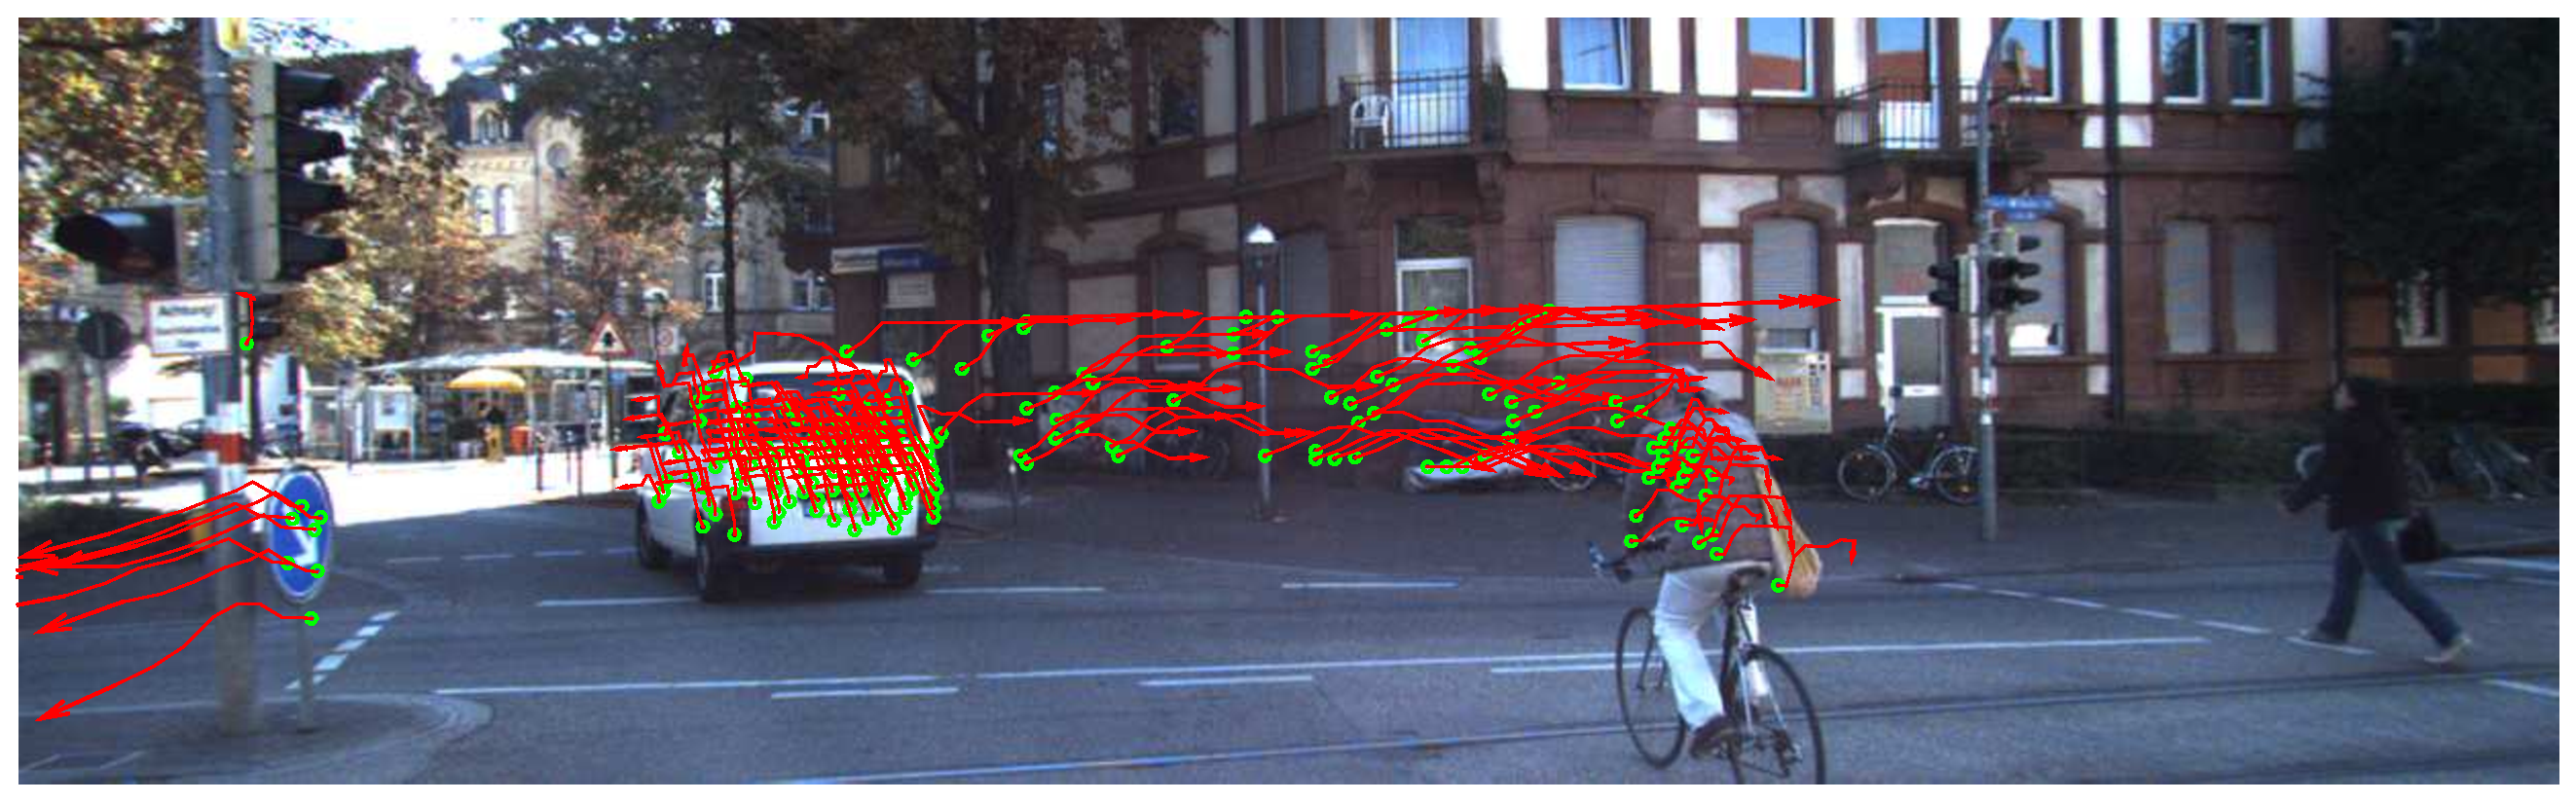
\includegraphics[height=0.108\textheight, width=0.98\textwidth]{image/traj2D.eps}%
  	\caption{2D feature trajectories.}
  	\label{fig:2dtraj}
	\end{subfigure}%
	\begin{subfigure}{0.5\textwidth}
 	\centering
  	\includegraphics[height=0.108\textheight, width=0.98\textwidth]{image/traj3D.eps}%{image/traj3D.png}
  	\caption{3D feature trajectories.}
  	\label{fig:3dtraj} 
  	\end{subfigure}%
  	
  \centering
	\begin{subfigure}{0.5\textwidth}
  	\centering
 	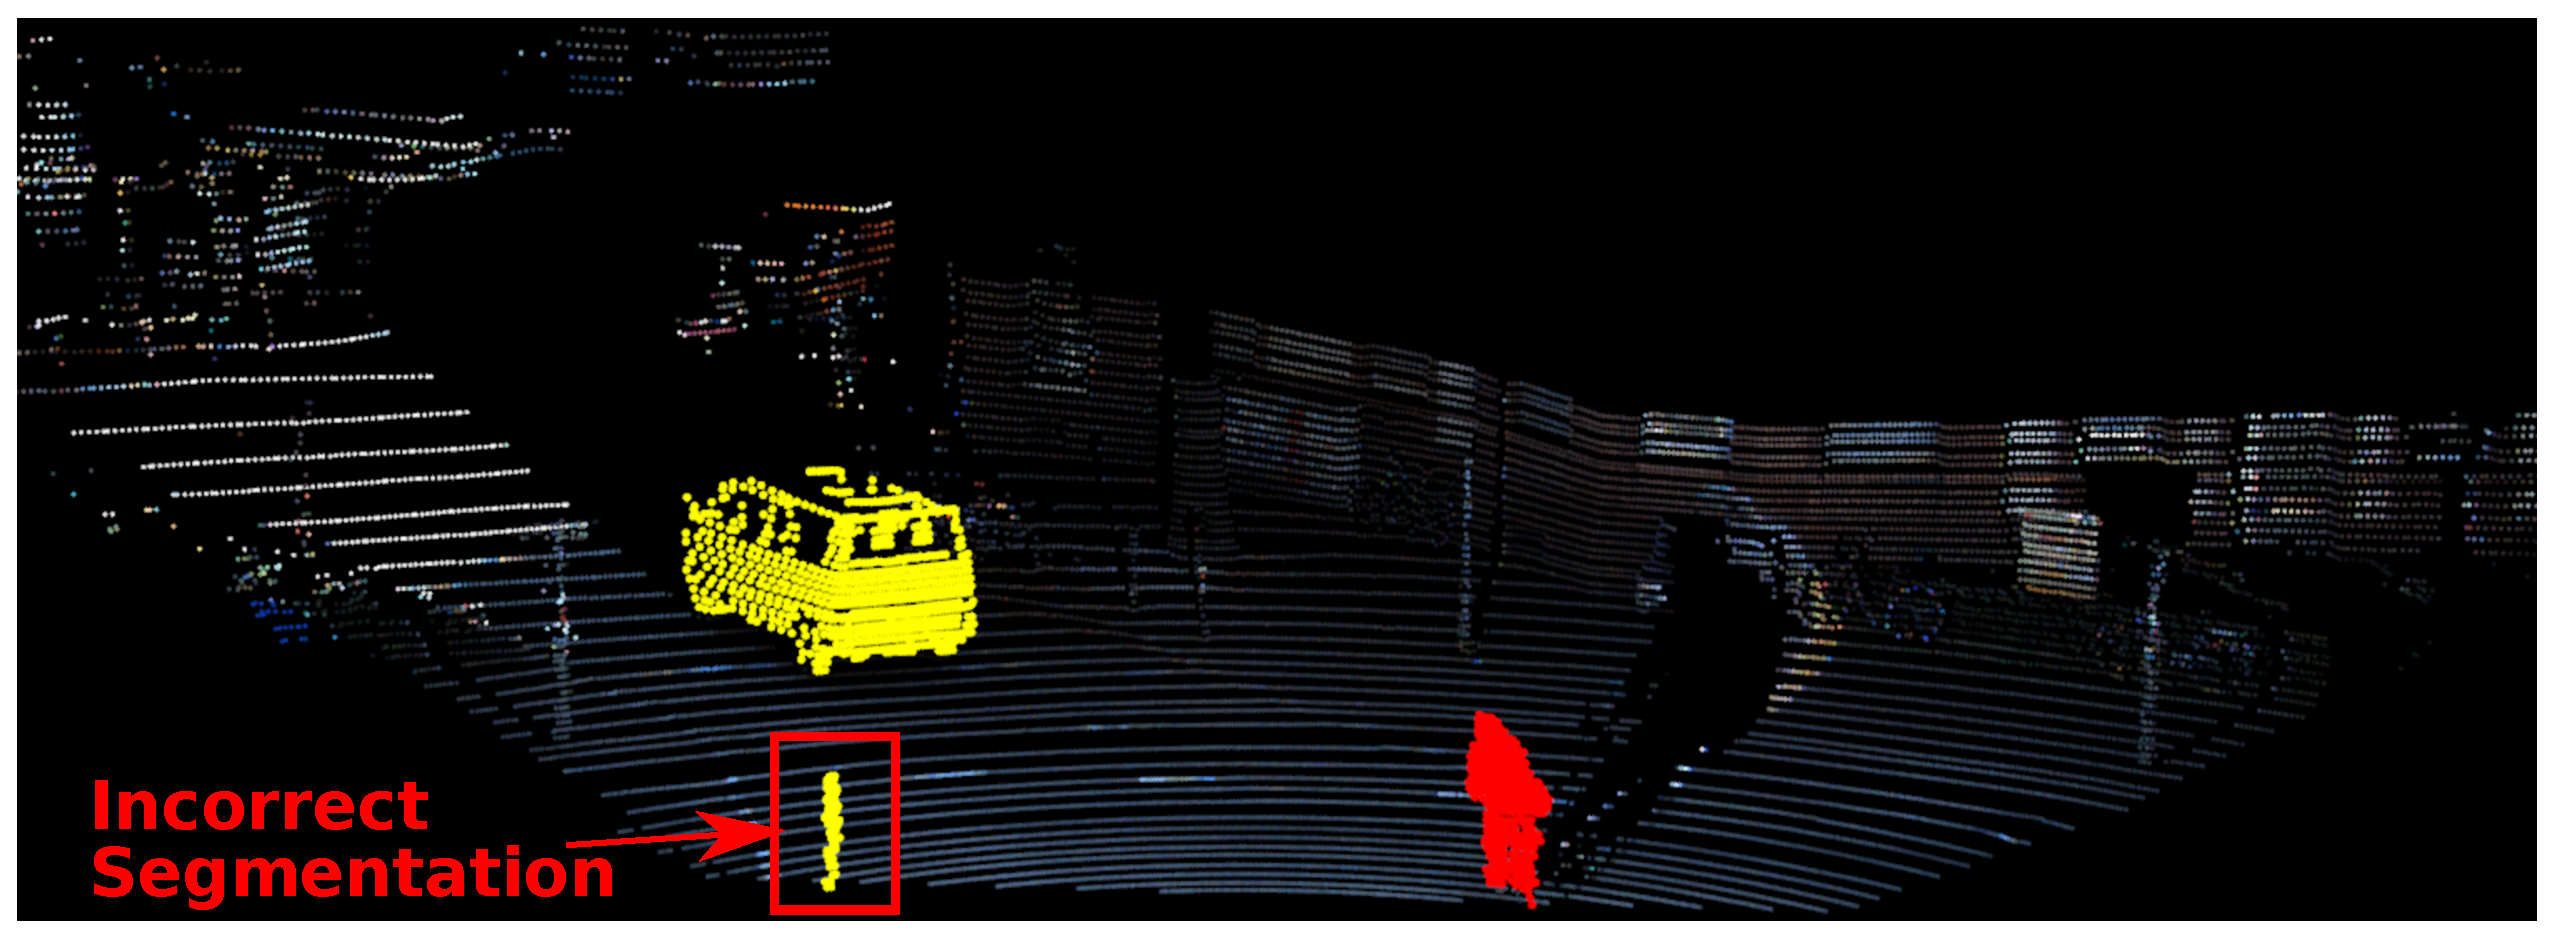
\includegraphics[height=0.108\textheight, width=0.98\textwidth]{image/MS2D_RG.eps}
  	\caption{ 3D Region growing segmentation based on 2D MS \cite{c2}.}
  	\label{fig:2dRG}
	\end{subfigure}%
	\begin{subfigure}{0.5\textwidth}
 	\centering
  	\includegraphics[height=0.108\textheight, width=0.98\textwidth]{image/MS3D_RG.eps}%{image/MS3D_RG.png}
  	\caption{3D Region growing segmentation based on our method.}
  	\label{fig:3dRG} 
  	\end{subfigure}%
\caption{2D vs. 3D MS results: (a) and (b) show the 2D and 3D feature trajectories from frame 1 to 10, respectively. Arrows in (a) represent the direction of the feature motions. (c) and (d) show the 3D region growing segmentation based on the segmented feature trajectories using 2D-SSC and our 3D-SSC algorithm, respectively. Must view in color.}
\label{fig:MSRG}
\vspace{-3mm}
\end{figure*}

%=================================================================================
%=================================================================================
\begin{figure*}[t]

  \centering
	\begin{subfigure}{0.5\textwidth}
  	\centering
 	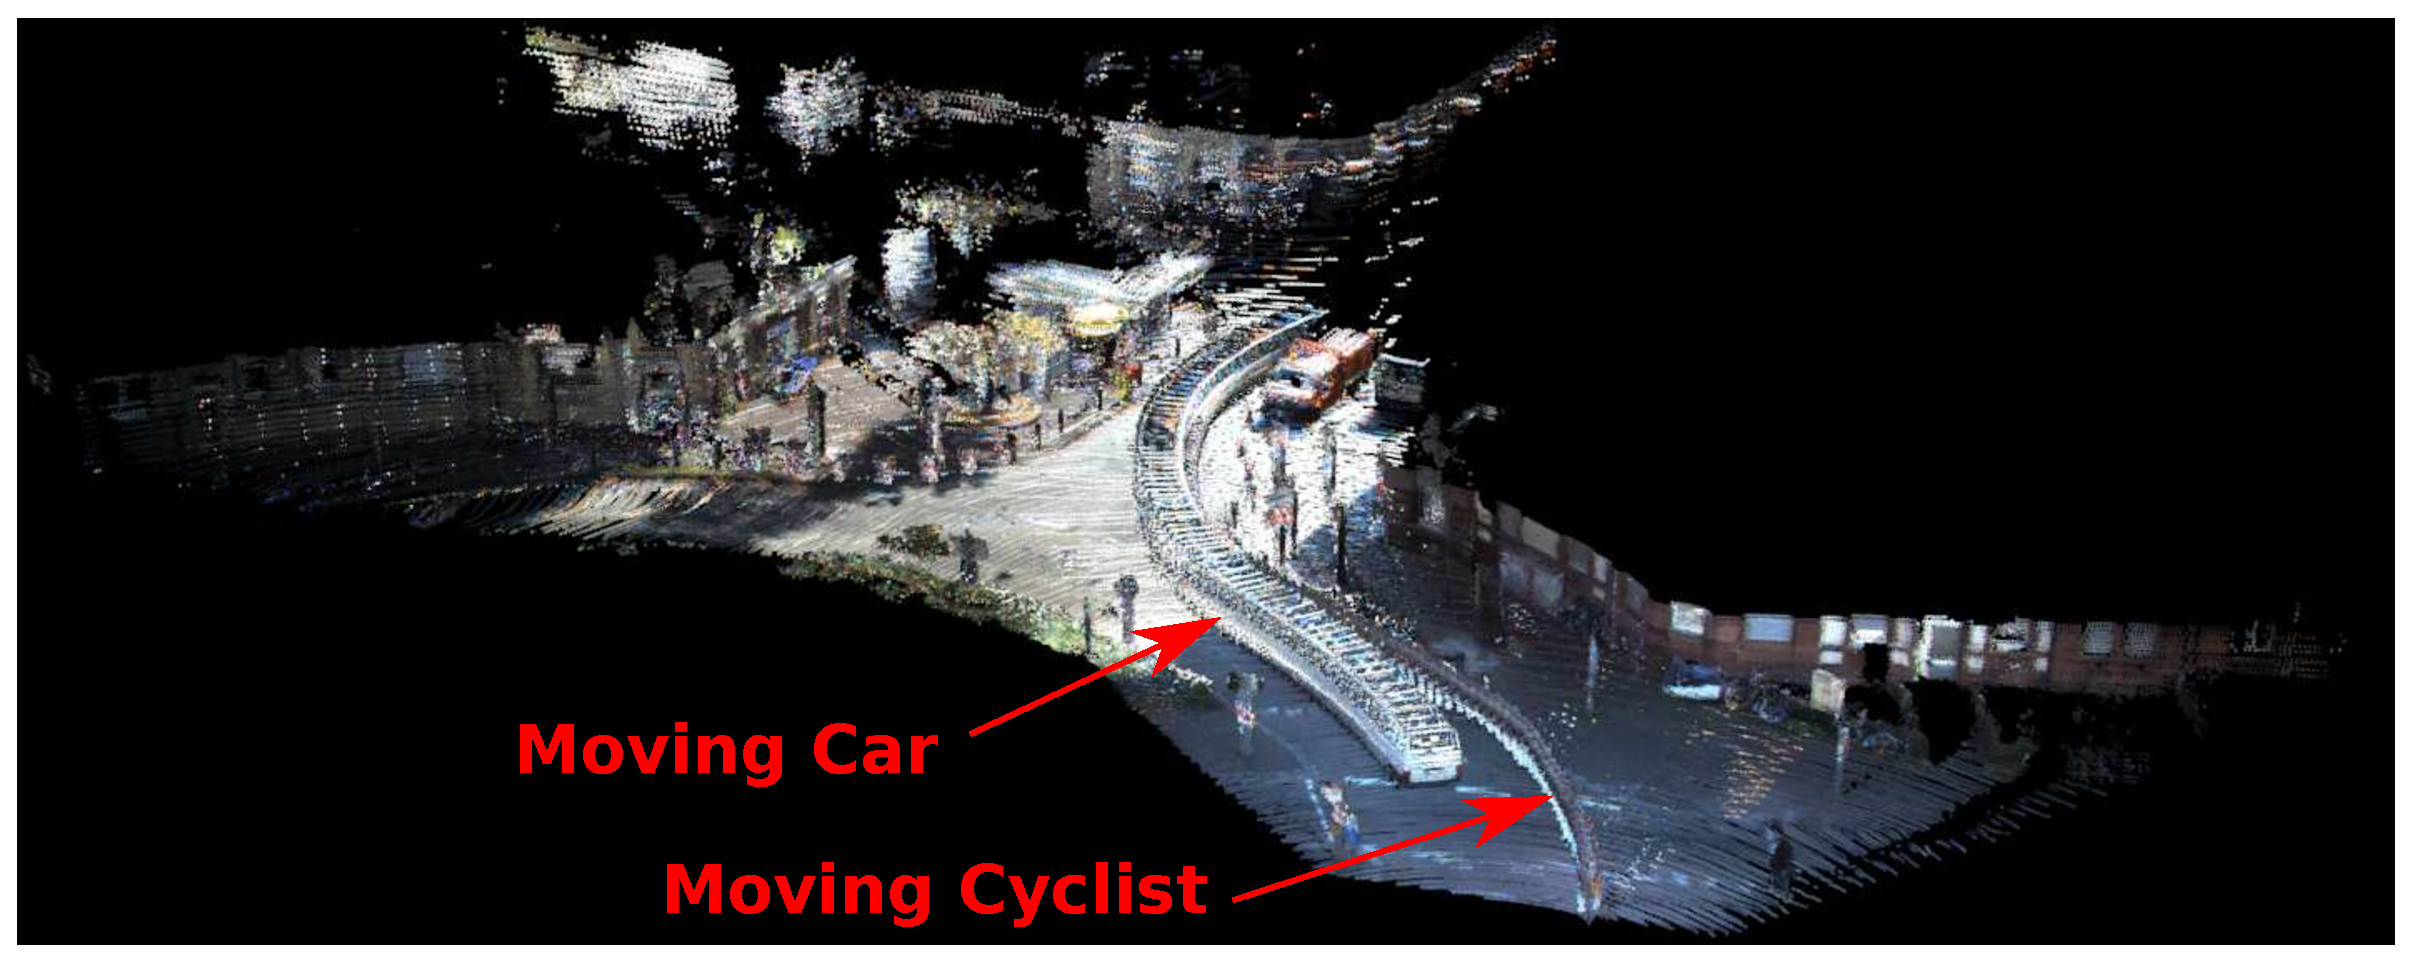
\includegraphics[height=0.12\textheight, width=0.98\textwidth]{image/seqRansac_Marked.eps}
  	\caption{Reconstructed full scene using \cite{c31}.}
  	\label{fig:seqRansac}
	\end{subfigure}%
	\begin{subfigure}{0.5\textwidth}
 	\centering
  	\includegraphics[height=0.12\textheight, width=0.98\textwidth]{image/static_map.eps}%{image/static_map.png}
  	\caption{Reconstructed static-map.}
  	\label{fig:static_map} 
  	\end{subfigure}%
  	
  \centering
    
    ~
  	\begin{subfigure}{0.165\textwidth}
 	\centering
  	\includegraphics[ width=1\textwidth]{image/000001.eps}%{image/000001.png}
  	\caption{Frame 1}
  	\label{fig:frame_1}
  	\end{subfigure}%
  	\begin{subfigure}{0.165\textwidth} 
 	\centering
  	\includegraphics[width=1\textwidth]{image/000015.eps}%{image/000015.png}
  	\caption{Frame 15}
  	\label{fig:frame_15}
  	\end{subfigure}%
  	\begin{subfigure}{0.165\textwidth} 
 	\centering
  	\includegraphics[width=1\textwidth]{image/000030.eps}%{image/000030.png}
  	\caption{Frame 30}
  	\label{fig:frame_30}
  	\end{subfigure}%
  	\begin{subfigure}{0.165\textwidth} 
 	\centering
  	\includegraphics[width=1\textwidth]{image/000045.eps}%{image/000045.png}
  	\caption{Frame 45}
  	\label{fig:frame_45}
  	\end{subfigure}%
  	\begin{subfigure}{0.165\textwidth} 
 	\centering
  	\includegraphics[width=1\textwidth]{image/000060.eps}%{image/000060.png}
  	\caption{Frame 60}
  	\label{fig:frame_60}
  	\end{subfigure}%
  	\begin{subfigure}{0.165\textwidth} 
 	\centering
  	\includegraphics[width=1\textwidth]{image/000075.eps}%{image/000075.png}
  	\caption{Frame 75}
  	\label{fig:frame_75}
  	\end{subfigure}%
\caption{Junction sequence results: (a) shows the full scene 3D reconstruction using 80 frames. (b) shows the reconstructed static-map without moving objects. (c)-(h) show the corresponding image sequence every 15 frames. Better view in color.}
\label{fig:car_static_map_Reconst}
\vspace{-3mm}
\end{figure*}


\begin{figure*}[t]
  \centering
  \begin{subfigure}{0.5\textwidth}
 	\centering
  	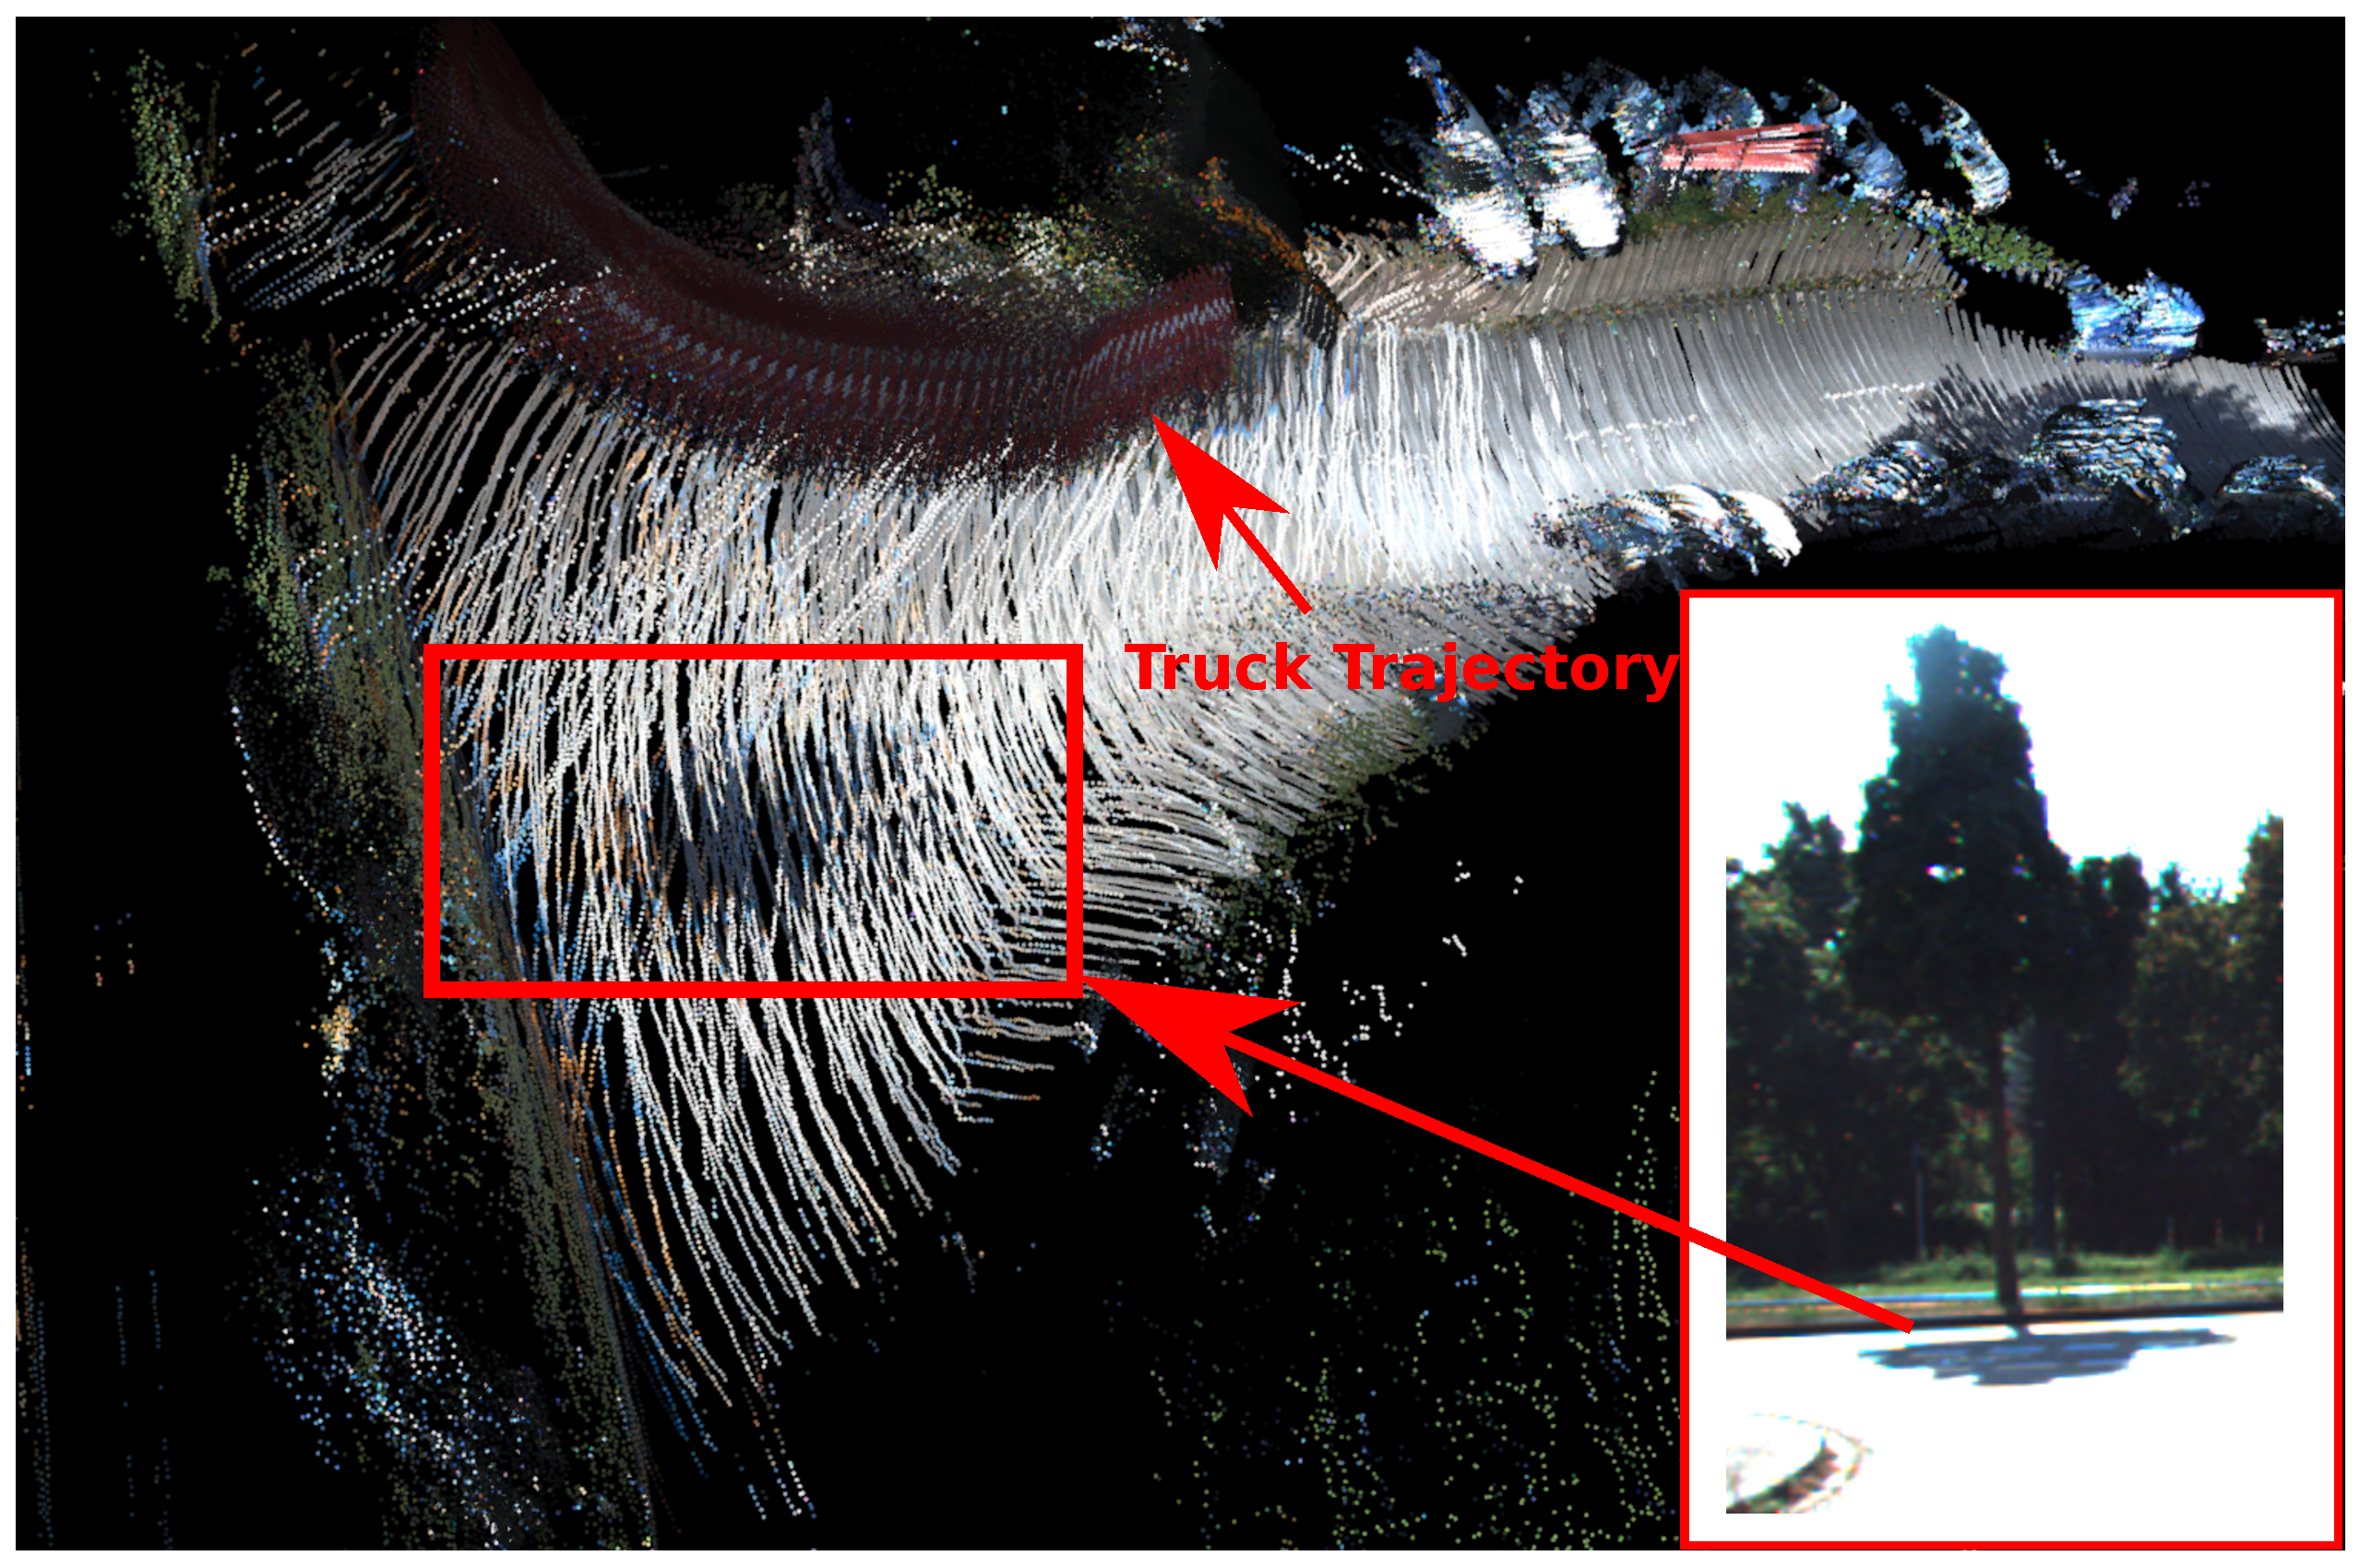
\includegraphics[height=0.24\textheight, width=0.98\textwidth]{image/truck_full_tree.eps}
  	\caption{Reconstructed full scene using \cite{c31}.}
  	\label{fig:truck_full_tree} 
  	\end{subfigure}%
	\begin{subfigure}{0.5\textwidth}
  	\centering
 	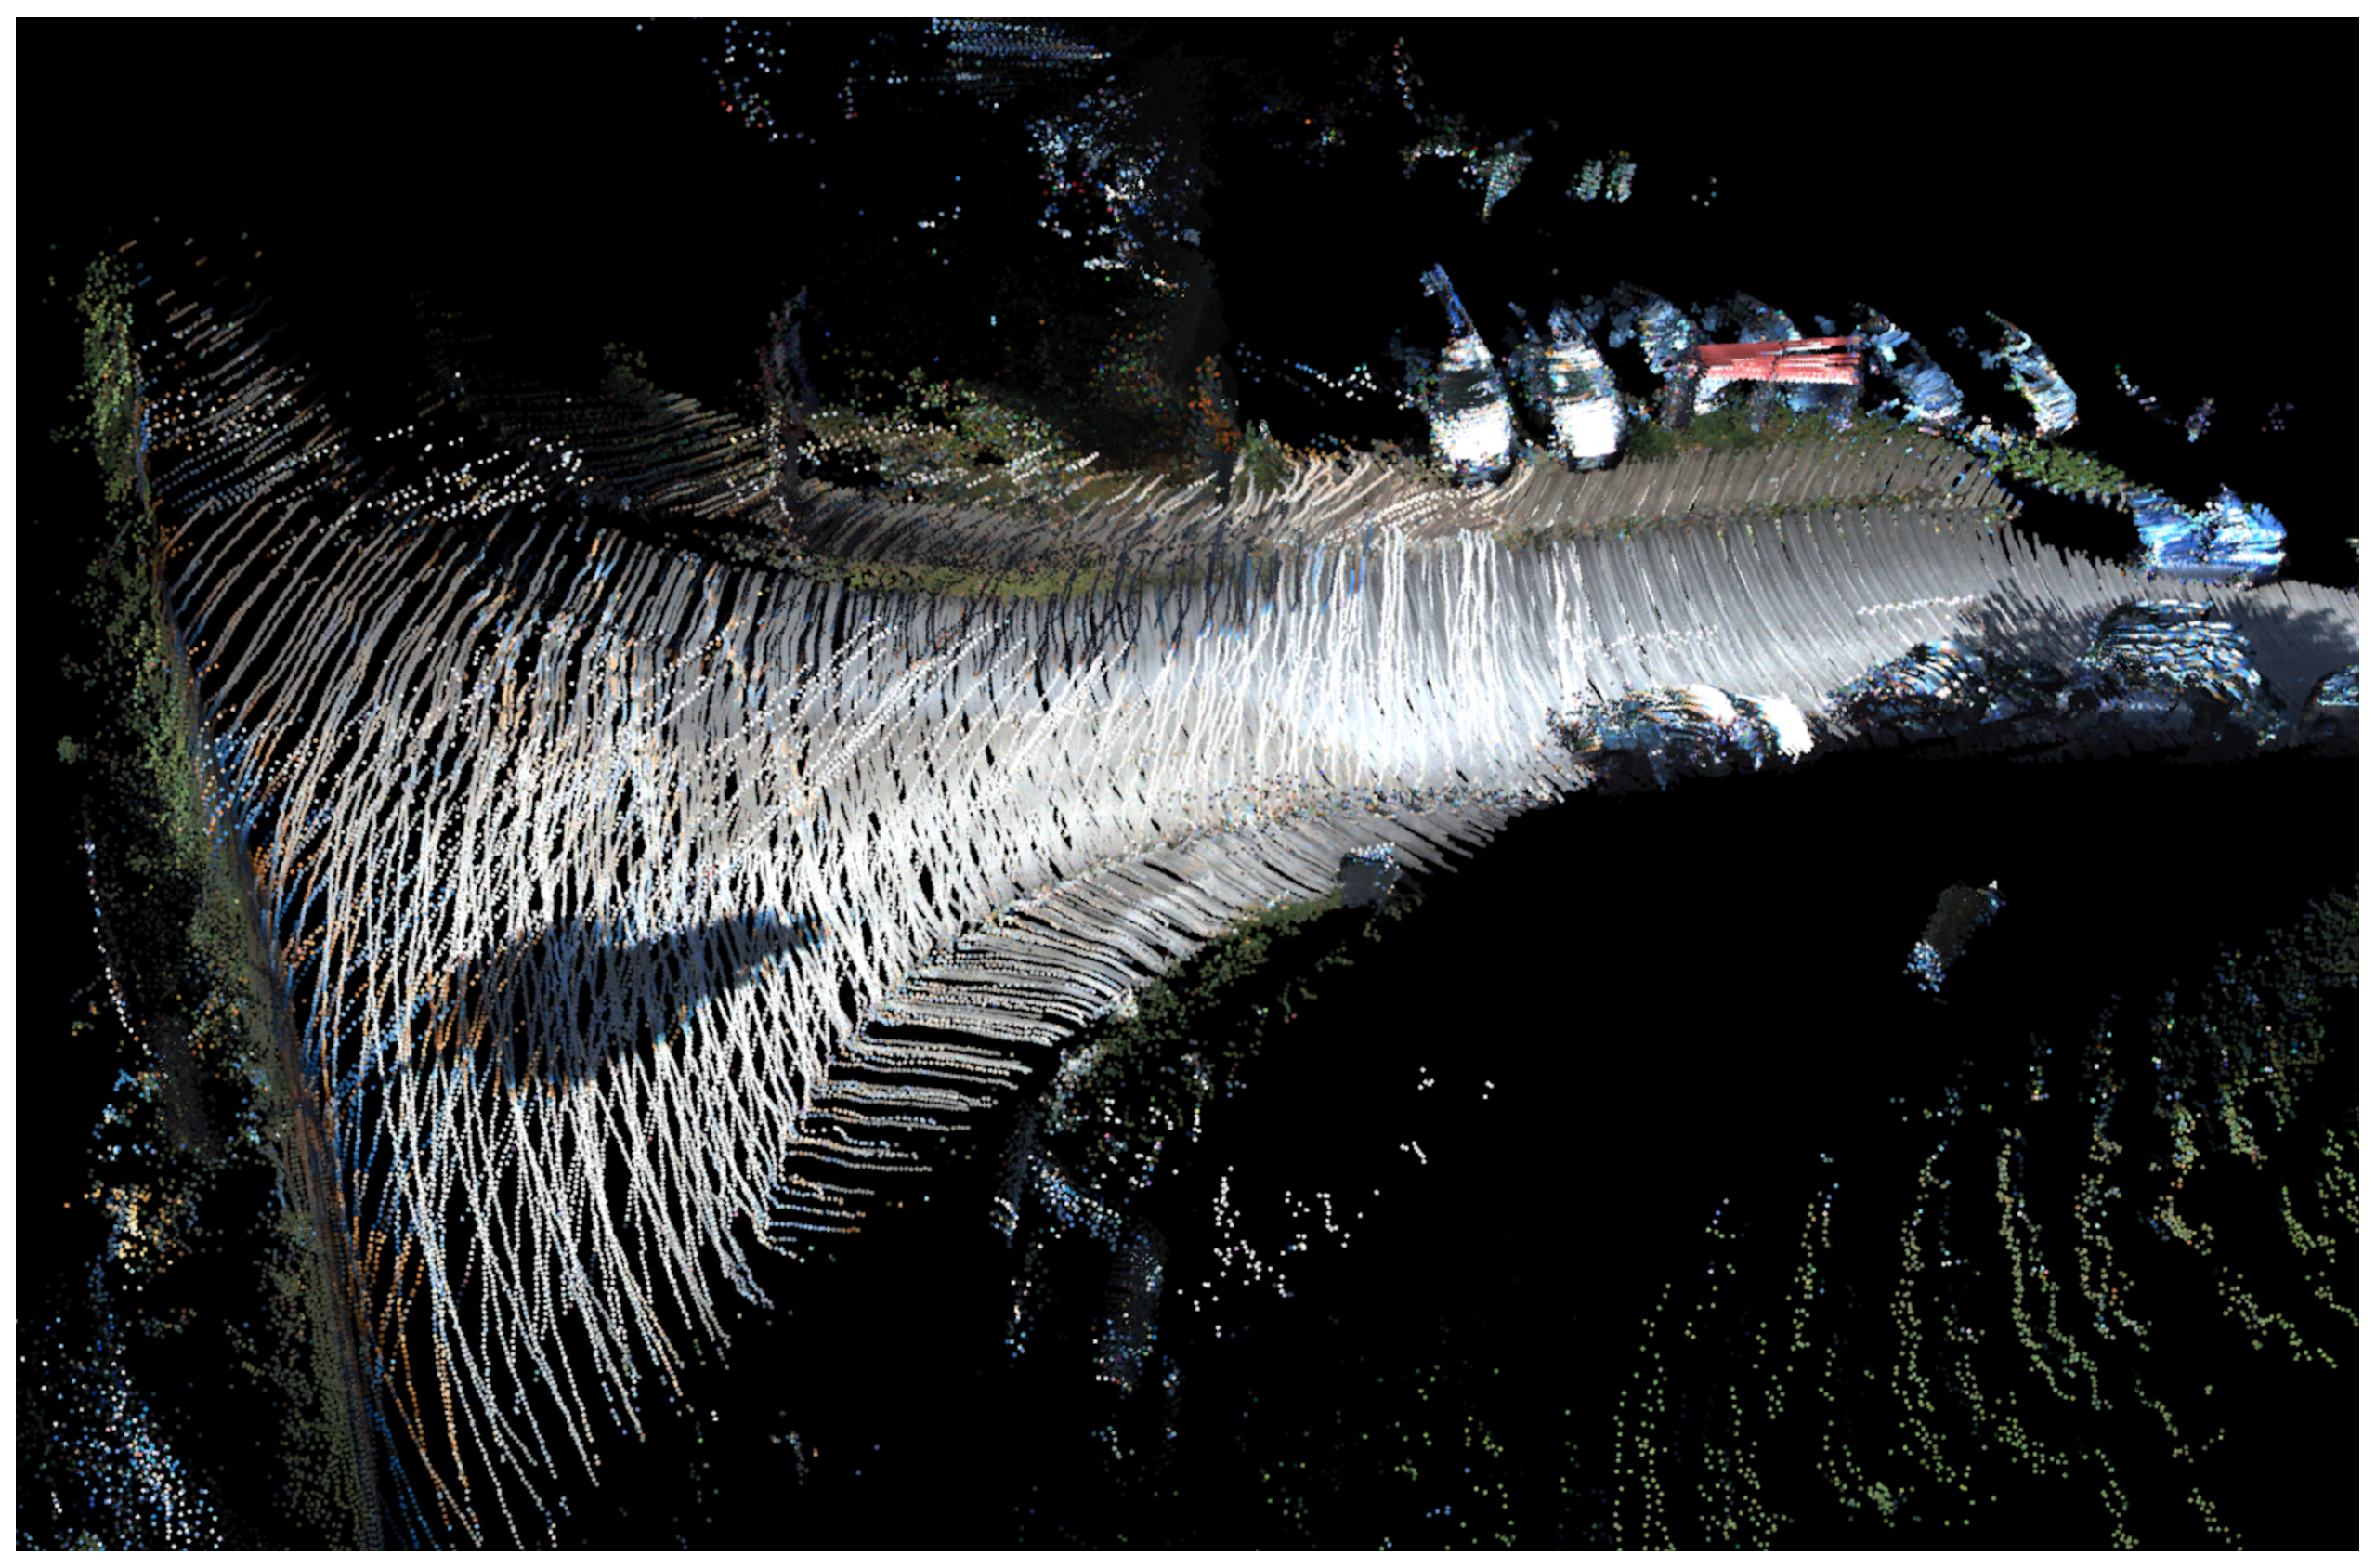
\includegraphics[height=0.24\textheight, width=0.98\textwidth]{image/truck_static_tree.eps}
  	\caption{Reconstructed static-scene.}
  	\label{fig:truck_static_tree}
	\end{subfigure}%
	
	
	\begin{subfigure}{0.2\textwidth}
 	\centering
  	\includegraphics[ width=1\textwidth]{image/000240.eps}%{image/000240.png}
  	\caption{Frame 1}
  	\label{fig:frame_1}
  	\end{subfigure}%
  	\begin{subfigure}{0.2\textwidth} 
 	\centering
  	\includegraphics[width=1\textwidth]{image/000250.eps}%{image/000250.png}
  	\caption{Frame 10}
  	\label{fig:frame_10}
  	\end{subfigure}%
  	\begin{subfigure}{0.2\textwidth} 
 	\centering
  	\includegraphics[width=1\textwidth]{image/000260.eps}%{image/000260.png}
  	\caption{Frame 20}
  	\label{fig:frame_20}
  	\end{subfigure}%
  	\begin{subfigure}{0.2\textwidth} 
 	\centering
  	\includegraphics[width=1\textwidth]{image/000270.eps}%{image/000270.png}
  	\caption{Frame 30}
  	\label{fig:frame_30}
  	\end{subfigure}%
  	\begin{subfigure}{0.2\textwidth} 
 	\centering
  	\includegraphics[width=1\textwidth]{image/000280.eps}%{image/000280.png}
  	\caption{Frame 40}
  	\label{fig:frame_40}
  	\end{subfigure}%
  	\caption{Highway sequence static-map reconstruction results: (a) shows the full scene 3D reconstruction using 45 frames. The red rectangle shows the reconstruction of tree shadow. (b) shows the reconstructed static-map without moving objects. (c)-(g) show the corresponding image sequence every 10 frames. Better view in color.}
\label{fig:truck_static_map_Reconst}
\vspace{-3mm}
\end{figure*}

\begin{figure*}
\vspace{-3mm}
  \centering
	\begin{subfigure}{0.333\textwidth}
  	\centering
 	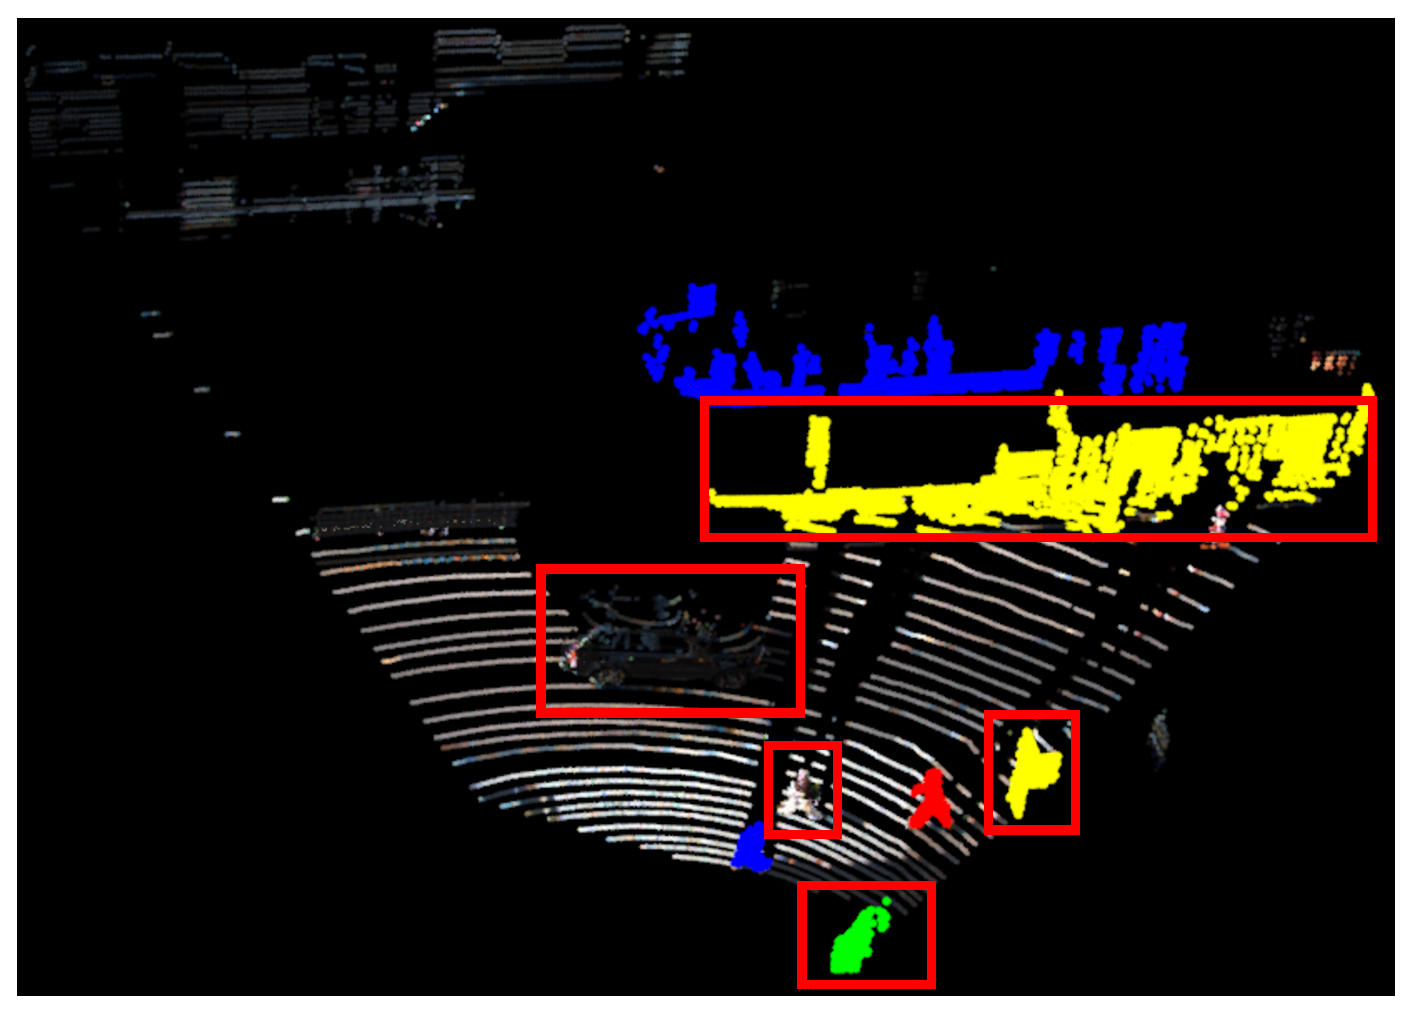
\includegraphics[height=0.17\textheight, width=0.98\textwidth]{image/train_MS2d_marked.eps}
  	\caption{2D-SSC MS result.}
  	\label{fig:train_MS2d_marked}
	\end{subfigure}%
	\begin{subfigure}{0.333\textwidth}
 	\centering
  	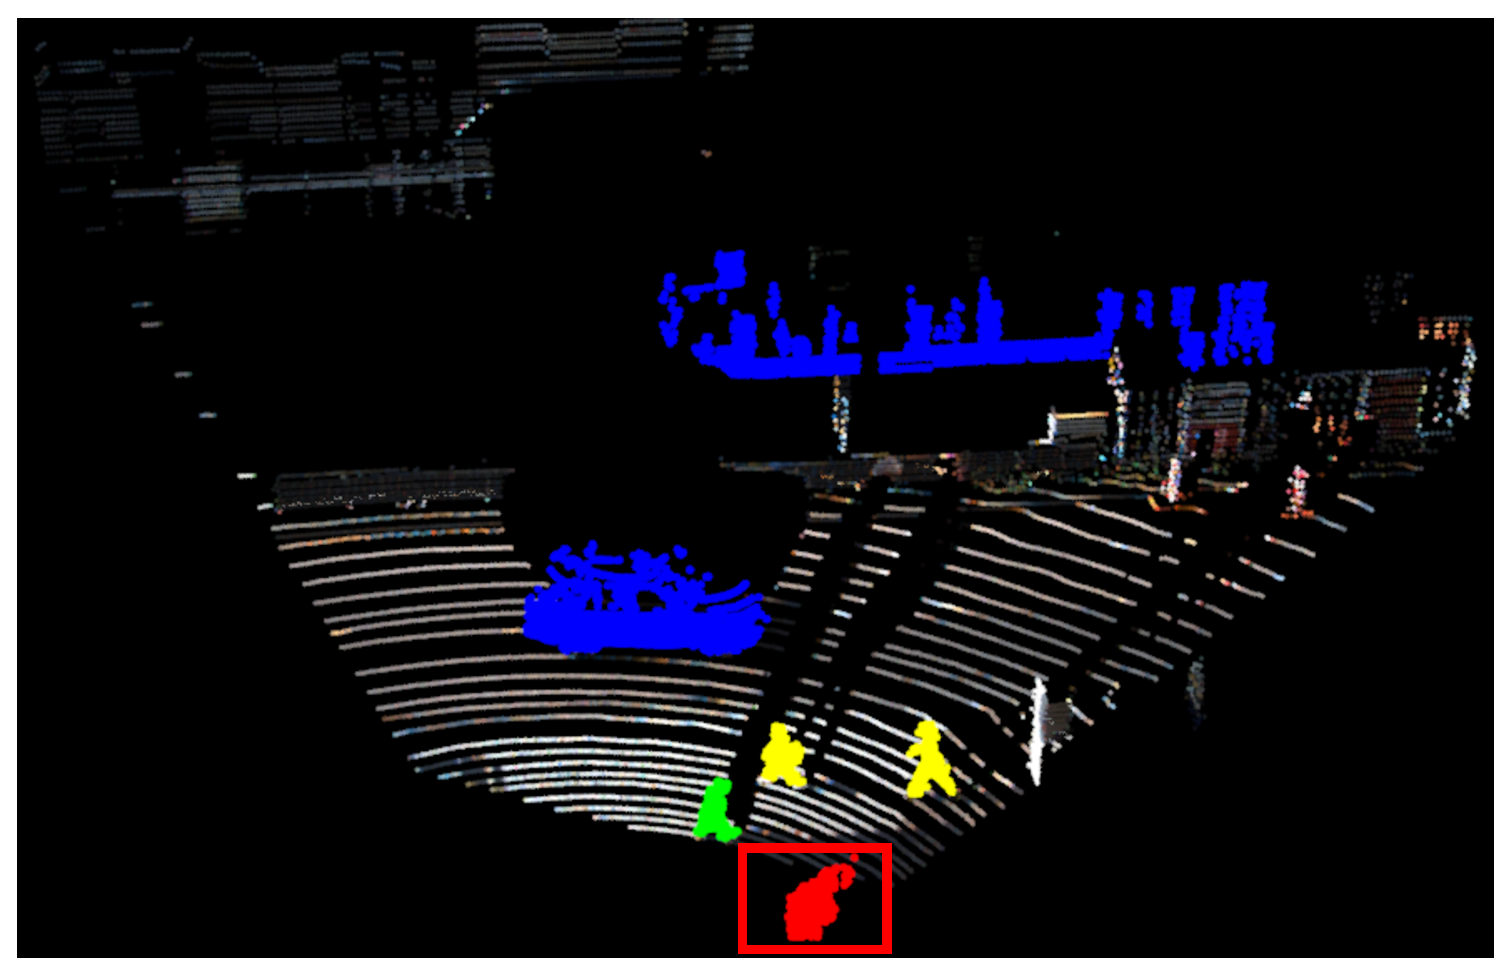
\includegraphics[height=0.17\textheight, width=0.98\textwidth]{image/train_MS3D_marked.eps}
  	\caption{Our 3D-SSC MS result.}
  	\label{fig:train_MS3D_marked} 
  	\end{subfigure}%
  	\begin{subfigure}{0.334\textwidth}
 	\centering
  	\includegraphics[height=0.17\textheight, width=0.98\textwidth]{image/train_static_view2_bright.eps}%{image/train_static_view2_bright.png}
  	\caption{Reconstructed static-map.}
  	\label{fig:train_static_view2} 
  	\end{subfigure}%
  	
  	
  	\begin{subfigure}{0.333\textwidth}
 	\centering
  	\includegraphics[ width=1\textwidth]{image/000940.eps}%{image/000940.png}
  	\caption{Frame 1}
  	\label{fig:frame_940}
  	\end{subfigure}%
  	\begin{subfigure}{0.333\textwidth} 
 	\centering
  	\includegraphics[width=1\textwidth]{image/000944.eps}%{image/000944.png}
  	\caption{Frame 5}
  	\label{fig:frame_944}
  	\end{subfigure}%
  	\begin{subfigure}{0.333\textwidth} 
 	\centering
  	\includegraphics[width=1\textwidth]{image/000948.eps}%{image/000948.png}
  	\caption{Frame 9}
  	\label{fig:frame_948}
  	\end{subfigure}%
  	\caption{Train station sequence static-map reconstruction results: (a) and (b) shows 2D-SSC and 3D-SSC MS results, respectively. Incorrect segmentations are highlighted with red rectangles. (c) shows the reconstructed static-map without moving objects from 9 frames. (d)-(f) show some selected corresponding sequential images.  Must view in color.}
\label{fig:train_static_map_Reconst}
\vspace{-3mm}
\end{figure*}


\section{Conclusion and Future Work}

We have proposed a novel framework for 3D motion segmentation using Sparse Subspace Clustering algorithm that categories the static scene parts and multiple moving objects. The proposed method has been tested with extensive experiments and outperforms its 2D based counterpart, especially when rich moving objects are involved. Our approach of sampling sparse feature trajectories based on their flow likelihood, and the proposed motion segmentation approach can handle wide range of motions, both in terms of magnitude and coverage. Furthermore, the proposed static-map building pipeline reconstructs photo-realistic maps, both for static and dynamic scene parts in an uncontrolled outdoor environment. In the future, more robust feature tracking algorithm, such as cross-frame optical flow, should be implemented to handle short-term occlusion problem. Also, multi-object trackers initialized with the detected moving objects should be developed to better understand the motions.

%update Yohan : avoid unnecessary control -> comment the next instruction
%\addtolength{\textheight}{-12cm}   % This command serves to balance the column lengths
                                  % on the last page of the document manually. It shortens
                                  % the textheight of the last page by a suitable amount.
                                  % This command does not take effect until the next page
                                  % so it should come on the page before the last. Make
                                  % sure that you do not shorten the textheight too much.

%%%%%%%%%%%%%%%%%%%%%%%%%%%%%%%%%%%%%%%%%%%%%%%%%%%%%%%%%%%%%%%%%%%%%%%%%%%%%%%%



%%%%%%%%%%%%%%%%%%%%%%%%%%%%%%%%%%%%%%%%%%%%%%%%%%%%%%%%%%%%%%%%%%%%%%%%%%%%%%%%



%%%%%%%%%%%%%%%%%%%%%%%%%%%%%%%%%%%%%%%%%%%%%%%%%%%%%%%%%%%%%%%%%%%%%%%%%%%%%%%%
% \section*{APPENDIX}

% Appendixes should appear before the acknowledgment.

% \section*{ACKNOWLEDGMENT}

% This project is funded by ...



%%%%%%%%%%%%%%%%%%%%%%%%%%%%%%%%%%%%%%%%%%%%%%%%%%%%%%%%%%%%%%%%%%%%%%%%%%%%%%%%
%update yohan, break page to force bib to be the last page
%\pagebreak
%\addtolength{\textheight}{-15cm}

\begin{thebibliography}{99}
\bibitem{c_1} Civera, J., Grasa, O., Davison, A. J., \& Montiel, J. 1‐Point RANSAC for extended Kalman filtering: Application to real‐time structure from motion and visual odometry. In Journal of Field Robotics, 2010.

\bibitem{c_2} Klein, G., \& Murray, D. Improving the agility of keyframe-based SLAM. In ECCV, 2008.

\bibitem{c0} Burgard, W., Stachniss, C., \& Hähnel, D. Mobile robot map learning from range data in dynamic environments. In Auto. Nav. in Dyn. Env., 2007.

\bibitem{c1} Tron, R., \& Vidal, R.. A benchmark for the comparison of 3-d motion segmentation algorithms. In CVPR, 2007. 

\bibitem{c2} Elhamifar, E., \& Vidal, R. Sparse subspace clustering: Algorithm, theory, and applications. In TPAMI, 2013.
%
%\bibitem{c5} Amaldi, E., \& Kann, V. On the approximability of minimizing nonzero variables or unsatisfied relations in linear systems. In Theoretical Computer Science, 1998.

\bibitem{c6} Rao, S., Tron, R., Vidal, R., \& Ma, Y. Motion segmentation in the presence of outlying, incomplete, or corrupted trajectories. In TPAMI, 2010.

%\bibitem{c7} Hartley R. and Zisserman, A., Multiple View Geometry in Computer Vision, Cambridge University Press, ISBN: 0521540518, 2004, pp 357-360.
%
%\bibitem{c8} Hartley R. and Vidal R., The multibody trifocal tensor: motion segmentation from 3 perspective views, CVPR, 2004, vol. 1, pp 769-775. 

\bibitem{c9} Vidal, R., \& Hartley, R. Motion segmentation with missing data using powerfactorization and gpca. In CVPR 2004.



%\bibitem{c10} Jingyu Y. and Marc P., A General Framework for Motion Segmentation: Independent, Articulated, Rigid, Non-rigid, Degenerate and Non-degenerate, ECCV, 2006, Vol. 3954, pp 94-106.
%
%\bibitem{c11} Fischler Martin A. and Bolles Robert C., Random Sample Consensus: A Paradigm for Model Fitting with Applications, ACM, 2004, vol 24 pp 381-395.

%\bibitem{c12} Vision Lab, Johns Hopkins University, Motion Segmentation in Dynamic Scenes, \url{ http://www.vision.jhu.edu/motion.php#results.}, 2012.

\bibitem{c13} Michael G. \& Stephen B., CVX: Matlab software for disciplined convex programming, version 2.0 beta, 2013.

\bibitem{c14} Ng, A. Y., Jordan, M. I., \& Weiss, Y. On spectral clustering: Analysis and an algorithm. In Adv. neural inf. proc. systems, 2002.

%\bibitem{c15} Duda Richard O., Peter E. Hart, and David G. Stork. Pattern classification. Wiley-Interscience, John Wiley \& Sons, 2012.

\bibitem{c16} Yan, J., \& Pollefeys, M. Articulated motion segmentation using ransac with priors. In Dynamical Vision, 2007.
%
%\bibitem{c17} Costeira  J. P. and T. Kanade, A multibody factorization method for independently moving objects, IJCV, Vol 29.3, 1998, pp 159-179.

\bibitem{c18}Stückler, J., \& Behnke, S. Efficient Dense Rigid-Body Motion Segmentation and Estimation in RGB-D Video. In IJCV, 2015.

\bibitem{c19} Sofer, Y., Hassner, T., \& Sharf, A. Interactive Learning for Point‐Cloud Motion Segmentation. In Computer Graphics Forum, 2013.

\bibitem{c20} Settles, B. Active learning literature survey. Tech. Report, 2010.

\bibitem{c21} Perera, S., Barnes, N., Xuming He, Izadi, S., Kohli, P., \& Glocker, B. Motion Segmentation of Truncated Signed Distance Function Based Volumetric Surfaces. In WACV, 2015.
%
%\bibitem{c22} David Hoag, Apollo Guidance and Navigation - Considerations of Apollo IMU Gimbal Lock, MIT Instrumentation Laboratory Document, 1963 E-1344.

\bibitem{c23} Cayley, A. About the algebraic structure of the orthogonal group and the other classical groups in a field of characteristic zero or a prime characteristic. In Reine Angewandte Mathematik, 1846.

\bibitem{c24}Liu, C., Yuen, J., Torralba, A., Sivic, J., \& Freeman, W. T. Sift flow: Dense correspondence across different scenes. In ECCV, 2008.

\bibitem{c25} Vosselman, G., Gorte, B. G., Sithole, G., \& Rabbani, T. Recognising structure in laser scanner point clouds. In Int. archives of photogrammetry, remote sensing and spatial information sciences, 2004.

\bibitem{c26}Wang, C., Thorpe, C., \& Thrun, S. Online simultaneous localization and mapping with detection and tracking of moving objects: Theory and results from a ground vehicle in crowded urban areas. In ICRA, 2003.

\bibitem{c27} Pomerleau, F., Krusi, P., Colas, F., Furgale, P., \& Siegwart, R. Long-term 3D map maintenance in dynamic environments. In ICRA, 2014.

\bibitem{c28} Ambrus, R., Bore, N., Folkesson, J., \& Jensfelt, P. Meta-rooms: Building and maintaining long term spatial models in a dynamic world. In IROS, 2014.

\bibitem{c30} Alismail, H., Baker, L. D., \& Browning, B. Continuous trajectory estimation for 3D SLAM from actuated lidar. In ICRA, 2014.

\bibitem{c31}Paudel, D. P., Demonceaux, C., Habed, A., Vasseur, P., \& Kweon, I. S. 2D-3D camera fusion for visual odometry in outdoor environments. In IROS, 2014.

\bibitem{c32} Geiger, A., Lenz, P., \& Urtasun, R. Are we ready for autonomous driving? the kitti vision benchmark suite. In CVPR, 2012.

\bibitem{c33} Fawcett, T. An introduction to ROC analysis. In Pattern recognition letters,  2006.

\pagebreak
\addtolength{\textheight}{-10cm}

\end{thebibliography}

\end{document}

%%% Local Variables:
%%% mode: latex
%%% TeX-master: t
%%% End:
